\documentclass[11pt, oneside]{article}   	% use "amsart" instead of "article" for AMSLaTeX format
\usepackage{geometry}                		% See geometry.pdf to learn the layout options. There are lots.
\usepackage{mathtools}
\usepackage{graphicx}
\usepackage{float}
\geometry{letterpaper}                   		% ... or a4paper or a5paper or ... 
%\geometry{landscape}                		% Activate for rotated page geometry
%\usepackage[parfill]{parskip}    		% Activate to begin paragraphs with an empty line rather than an indent
\usepackage{graphicx}				% Use pdf, png, jpg, or eps§ with pdflatex; use eps in DVI mode
								% TeX will automatically convert eps --> pdf in pdflatex		
\usepackage{amssymb}
\DeclareMathOperator{\Tr}{Tr}

%SetFonts

%SetFonts
\begin{document}

\title{Bi-Directional Training in Interference Network}

\author{Shao-Han Chen}
%\date{}							% Activate to display a given date or no date


\maketitle
%\section{}
%\subsection{}



\section{System Model 1: Private and Common Messages}

Under this model, we want to see how cooperation on transmitter(base station) side will improve the channel capacity. One way we implement the cooperation scheme is to make all transmitters for common messages, instead of working separately, a big cooperative array. That is to say, for the backward training part, we \textbf{minimize the mean square error(MSE) of total received signals together}. However, we found this method is actually \textbf{worse} than the one without cooperation. \textbf{How Doesn't this Work?} This is related the way we \textbf{measure performance}. Our objective is to maximize the \textbf{sum capacity} of individual users, which is equal to minimize $\displaystyle\sum_{k} MSE_{k}$. However, our cooperation scheme actually leads to the solution of maximizing total capacity, that is minimize $MSE$. Please note that we are not claiming cooperations imply worse performance. It's just this particular cooperation scheme doesn't work. 
\subsection{System Model}

\begin{figure}[h]
    \centering
    \centerline{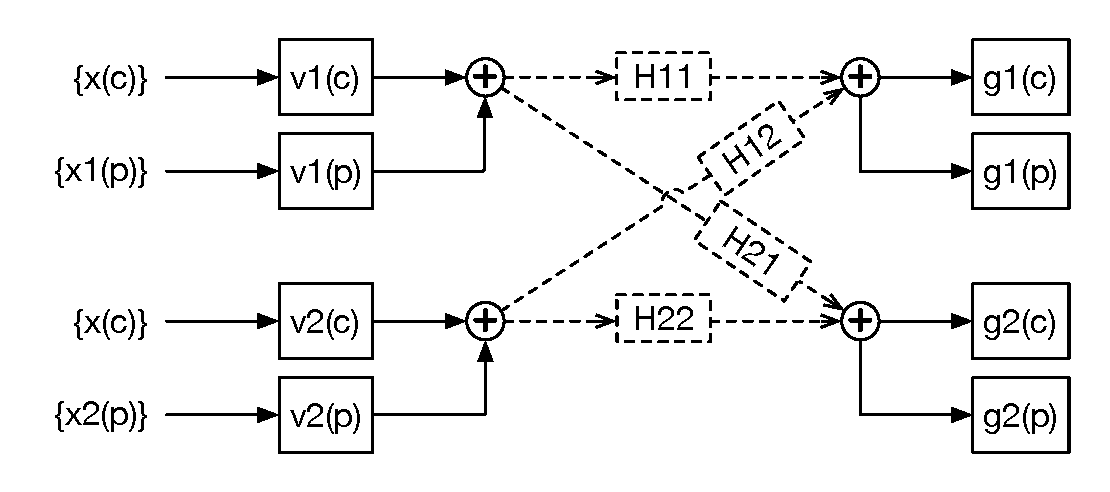
\includegraphics[width=110mm]{forward_channel}}
    \caption{Forward Channel}
\end{figure} 

\begin{figure}[h]
    \centering
    \centerline{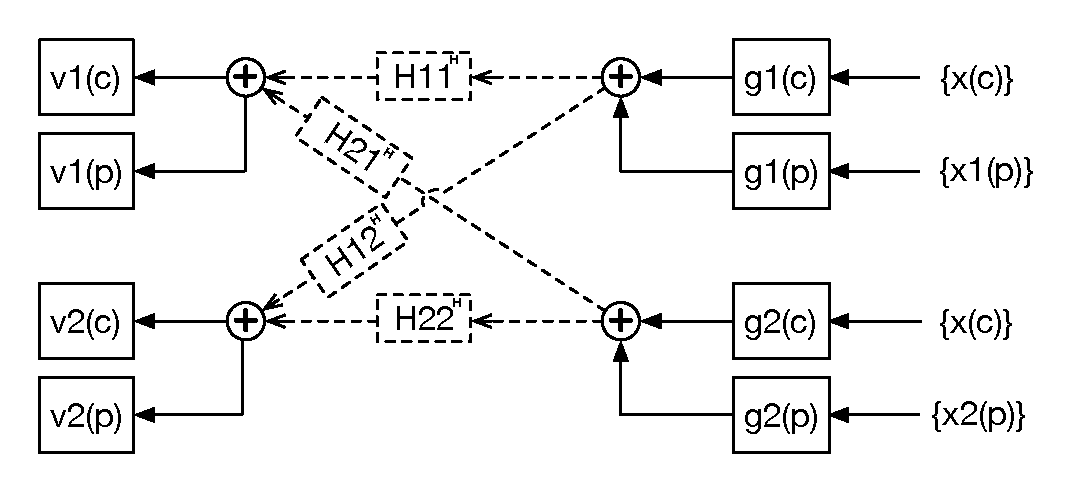
\includegraphics[width=110mm]{backward_channel}}
    \caption{Backward Channel}
\end{figure} 

\newpage

\subsection{Optimization Problem}
\begin{align*}
\min_{\textbf{v}_{k} ,\textbf{g}_{k}} \displaystyle\sum_{k} MSE^{(c)}_{k}+MSE^{(p)}_{k}
\end{align*}

\begin{align*}
\text{subject to}  \ 	\|	\textbf{v}^{(c)}_{k}	\|^{2}	+\|	\textbf{v}^{(p)}_{k}\|^{2}= P; \| \textbf{g}_{k}	\|^{2} = P
\end{align*}

where
\begin{align*}
MSE^{(c)}_{k} = \mathrm{E}	[	(	x-\textbf{g}^{H(c)}_{k}	\textbf{y}_{k}	)(x-\textbf{g}^{H(c)}_{k}	\textbf{y}_{k})^{H}	]
\end{align*}

\begin{align*}
MSE^{(p)}_{k} = \mathrm{E}	[	(	x^{(p)}_{k}-\textbf{g}^{H(p)}_{k}	\textbf{y}_{k}	)(x^{(p)}_{k}-\textbf{g}^{H(p)}_{k}	\textbf{y}_{k})^{H}	]
\end{align*}





\subsection{The received signal vector at k-th receiver}
\begin{align*}
\textbf{y}_{k} &= \textbf{H}_{kk}
			(\textbf{v}^{(c)}_{k}x
			+\textbf{v}^{(p)}_{k}x^{(p)}_{k})
			+\displaystyle\sum_{j \neq k}\textbf{H}_{kj}(\textbf{v}^{(c)}_{j}x+\textbf{v}^{(p)}_{j}x^{(p)}_{j})
			+\textbf{n}_{k}
\end{align*}

\subsection{SINR Derivation}
\begin{align*}
s^{(c)}_{k} = \textbf{g}^{H(c)}_{k}
		(\displaystyle\sum_{i}
		\textbf{H}_{ki} 
		\textbf{v}^{(c)}_{i}x)
\end{align*}

\begin{align*}
s^{(p)}_{k} = \textbf{g}^{H(p)}_{k}
		(\textbf{H}_{kk} 
		\textbf{v}^{(p)}_{k}x^{(p)}_{k})
\end{align*}

\begin{align*}
n^{(c)}_{k} = \textbf{g}^{H(c)}_{k}
		(\displaystyle\sum_{i}
		\textbf{H}_{ki} 
		\textbf{v}^{(p)}_{i}x^{(p)}_{i}
		+\textbf{n}_{k})
\end{align*}

\begin{align*}
n^{(p)}_{k} = \textbf{g}^{H(p)}_{k}
		(\displaystyle\sum_{i}
		\textbf{H}_{ki} 
		\textbf{v}^{(c)}_{i}x
		+\displaystyle\sum_{j \neq k}\textbf{H}_{kj}\textbf{v}^{(p)}_{j}x^{(p)}_{j}
		+\textbf{n}_{k})
\end{align*}

\begin{align*}
\frac	{	|s^{(c)}_{k}|^2	}{	|n^{(c)}_{k}|^2	} = 
\frac {	|\textbf{g}^{H(c)}_{k}
		\displaystyle\sum_{i}
		\textbf{H}_{ki} 
		\textbf{v}^{(c)}_{i}|^2	
	} 
	{	\displaystyle\sum_{i}
		|\textbf{g}^{H(c)}_{k}
		\textbf{H}_{ki} 
		\textbf{v}^{(p)}_{i}|^2
		+|\textbf{g}^{H(c)}_{k}
		\textbf{R}_{k}
		\textbf{g}^{(c)}_{k}|
	}
\end{align*}

\begin{align*}
\frac	{	|s^{(p)}_{k}|^2	}{	|n^{(p)}_{k}|^2	} = 
\frac {|\textbf{g}^{H(p)}_{k}
		\textbf{H}_{kk} 
		\textbf{v}^{(p)}_{k}|^2	
	} 
	{	|\textbf{g}^{H(p)}_{k}
		\displaystyle\sum_{i}
		\textbf{H}_{ki} 
		\textbf{v}^{(c)}_{i}|^2
		+\displaystyle\sum_{j \neq k}
		|\textbf{g}^{H(p)}_{k}
		\textbf{H}_{kj} 
		\textbf{v}^{(p)}_{j}|^2
		+|\textbf{g}^{H(p)}_{k}
		\textbf{R}_{k}
		\textbf{g}^{(p)}_{k}|
	}
\end{align*}

\subsection{Max-SINR Algorithm[Gomadam, 2011]}
For Max-SINR algorithm, we assume \textbf{all channel state information(CSI) is available} to each user. In this method, the solution for each transceivers  are simply Wiener filters. In other words, solving it by Wiener-Hopf equation: $R^{-1}p$ [Adaptive Filter Theory, Simon Haykin]

\subsubsection{Forward\ Training (fix $\textbf{v}^{(c)}_{k}$, $\textbf{v}^{(p)}_{k}$, $\forall k$)}


\begin{align*}
\textbf{g}^{*(c)}_{k} = 
&\bigg[
\textbf{H}_{kk}	\textbf{v}^{(c)}_{k}	\textbf{v}^{H(c)}_{k}	\textbf{H}^{H}_{kk}
+\textbf{H}_{kk}	\textbf{v}^{(p)}_{k}	\textbf{v}^{H(p)}_{k}	\textbf{H}^{H}_{kk}	\\
&+(\displaystyle\sum_{j \neq k}\textbf{H}_{kj}\textbf{v}^{(c)}_{j})
(\displaystyle\sum_{j \neq k}\textbf{v}^{H(c)}_{j}\textbf{H}^{H}_{kj})
+(\displaystyle\sum_{j \neq k}\textbf{H}_{kj}\textbf{v}^{(p)}_{j} \textbf{v}^{H(p)}_{j}\textbf{H}^{H}_{kj})	\\
&+\textbf{H}_{kk}	\textbf{v}^{(c)}_{k}
(\displaystyle\sum_{j \neq k}\textbf{v}^{H(c)}_{j}\textbf{H}^{H}_{kj})
+(\displaystyle\sum_{j \neq k}\textbf{H}_{kj}\textbf{v}^{(c)}_{j})
\textbf{v}^{H(c)}_{k}	\textbf{H}^{H}_{kk}
+\sigma^2	\textbf{I}
\bigg]^{-1}	 	(\displaystyle\sum_{i}	\textbf{H}_{ki} 	\textbf{v}^{(c)}_{i})	
\end{align*}

\begin{align*}
\textbf{g}^{*(p)}_{k} = 	
&\bigg[
\textbf{H}_{kk}	\textbf{v}^{(c)}_{k}	\textbf{v}^{H(c)}_{k}	\textbf{H}^{H}_{kk}
+\textbf{H}_{kk}	\textbf{v}^{(p)}_{k}	\textbf{v}^{H(p)}_{k}	\textbf{H}^{H}_{kk}	\\
&+(\displaystyle\sum_{j \neq k}\textbf{H}_{kj}\textbf{v}^{(c)}_{j})
(\displaystyle\sum_{j \neq k}\textbf{v}^{H(c)}_{j}\textbf{H}^{H}_{kj})
+(\displaystyle\sum_{j \neq k}\textbf{H}_{kj}\textbf{v}^{(p)}_{j} \textbf{v}^{H(p)}_{j}\textbf{H}^{H}_{kj})	\\
&+\textbf{H}_{kk}	\textbf{v}^{(c)}_{k}
(\displaystyle\sum_{j \neq k}\textbf{v}^{H(c)}_{j}\textbf{H}^{H}_{kj})
+(\displaystyle\sum_{j \neq k}\textbf{H}_{kj}\textbf{v}^{(c)}_{j})
\textbf{v}^{H(c)}_{k}	\textbf{H}^{H}_{kk}
+\sigma^2	\textbf{I}
\bigg]^{-1}	 (\textbf{H}_{kk} 	\textbf{v}^{(p)}_{k})
\end{align*}


\subsubsection{Backward\ Training (fix\  $\textbf{g}^{(c)}_{k}$, $\textbf{g}^{(p)}_{k}$, $\forall k$)}


\begin{align*}
\textbf{Z}_{ab}=\textbf{H}^{H}_{ba} 
\end{align*}

\paragraph{without cooperation}


\begin{align*}
\textbf{v}^{*(c)}_{k} = 
&\bigg[
\textbf{Z}_{kk}	\textbf{g}^{(c)}_{k}	\textbf{g}^{H(c)}_{k}	\textbf{Z}^{H}_{kk}
+\textbf{Z}_{kk}	\textbf{g}^{(p)}_{k}	\textbf{g}^{H(p)}_{k}	\textbf{Z}^{H}_{kk}	\\
&+(\displaystyle\sum_{j \neq k}\textbf{Z}_{kj}\textbf{g}^{(c)}_{j})
(\displaystyle\sum_{j \neq k}\textbf{g}^{H(c)}_{j}\textbf{Z}^{H}_{kj})
+(\displaystyle\sum_{j \neq k}\textbf{Z}_{kj}\textbf{g}^{(p)}_{j}	\textbf{g}^{H(p)}_{j}\textbf{Z}^{H}_{kj})	\\
&+\textbf{Z}_{kk}	\textbf{g}^{(c)}_{k}
(\displaystyle\sum_{j \neq k}\textbf{g}^{H(c)}_{j}\textbf{Z}^{H}_{kj})
+(\displaystyle\sum_{j \neq k}\textbf{Z}_{kj}\textbf{g}^{(c)}_{j})
\textbf{g}^{H(c)}_{k}	\textbf{Z}^{H}_{kk}
+\sigma^2	\textbf{I}
\bigg]
^{-1}	 (	\displaystyle\sum_{i}   \textbf{Z}_{ki} 	\textbf{g}^{(c)}_{i}	)
\end{align*}






\paragraph{with cooperation}


\begin{align*}
\textbf{V}^{*(c)} =  		
&\left\{ 
\textbf{[Z]}	\textbf{g}^{(c)}	\textbf{g}^{H(c)}		\textbf{[Z]}^{H}
+\textbf{[Z]}
\begin{bmatrix}
       \textbf{g}^{(p)}_{1}	\textbf{g}^{H(p)}_{1} &  &   \textbf{O}      \\[0.3em]
        & \ddots       & \\[0.3em]
           \textbf{O}        & & \textbf{g}^{(p)}_{k}	\textbf{g}^{H(p)}_{k}
     \end{bmatrix}
    \textbf{[Z]}^{H}
    +\sigma^2	\textbf{I}
\right\}
^{-1} ( \textbf{[Z]}  \textbf{g}^{(c)}	)	
\end{align*}

\begin{align*}
\textbf{v}^{*(p)}_{k} =	
 &\bigg[
\textbf{Z}_{kk}	\textbf{g}^{(c)}_{k}	\textbf{g}^{H(c)}_{k}	\textbf{Z}^{H}_{kk}
+\textbf{Z}_{kk}	\textbf{g}^{(p)}_{k}	\textbf{g}^{H(p)}_{k}	\textbf{Z}^{H}_{kk}	\\
&+(\displaystyle\sum_{j \neq k}\textbf{Z}_{kj}\textbf{g}^{(c)}_{j})
(\displaystyle\sum_{j \neq k}\textbf{g}^{H(c)}_{j}\textbf{Z}^{H}_{kj})
+(\displaystyle\sum_{j \neq k}\textbf{Z}_{kj}\textbf{g}^{(p)}_{j}	\textbf{g}^{H(p)}_{j}\textbf{Z}^{H}_{kj})	\\
&+\textbf{Z}_{kk}	\textbf{g}^{(c)}_{k}
(\displaystyle\sum_{j \neq k}\textbf{g}^{H(c)}_{j}\textbf{Z}^{H}_{kj})
+(\displaystyle\sum_{j \neq k}\textbf{Z}_{kj}\textbf{g}^{(c)}_{j})
\textbf{g}^{H(c)}_{k}	\textbf{Z}^{H}_{kk}
+\sigma^2	\textbf{I}
\bigg]^{-1}	 (\textbf{Z}_{kk}  \textbf{g}^{(p)}_{k})
\end{align*}

\subsection{Bi-Directional Training with LS Algorithm[Shi, 2014]}
For Bi-Directional Training, we assume \textbf{all channel state information(CSI) is not available} to each user. In this case, we could either adopt Least Mean Square Method(LMS) or Least Square Method(LS) to carry out the solution[Adaptive Filter Theory, Simon Haykin]. \textbf{There is actually another interesting finding here}. We all have seen the monotonically decreasing diagram of MSE when designing/studying filters with both methods. We can also show that when the filter converges(achieve minimum MSE), it also maximizes Signal to Interference plus Noise Ratio(SINR). \textbf{However, how does the SINR behave before it converges?} For LS, it is monotonically  decreasing just as MSE diagram, but for LMS, it is \textbf{not!} Therefore, LMS isn't applicable for our application. We need SINR increases after each iteration.


\subsubsection{Forward\ Training (fix\  $\textbf{v}^{(c)}_{k}$, $\textbf{v}^{(p)}_{k}$, $\forall k)$}


\begin{align*}
\textbf{g}^{(c)}_{k}(n+1)= \textbf{g}^{(c)}_{k}(n)+ \mu \textbf y_k(n) [x(n)- \textbf{g}^{H(c)}_{k}(n) \textbf y_k(n)]^*
\end{align*}

\begin{align*}
\textbf{g}^{(p)}_{k}(n+1)= \textbf{g}^{(p)}_{k}(n)+ \mu \textbf y_k(n) [x_k^{(p)}(n)- \textbf{g}^{H(p)}_{k}(n) \textbf y_k(n)]^*
\end{align*}


\subsubsection{Backward\ Training (fix\  $\textbf{g}^{(c)}_{k}$, $\textbf{g}^{(p)}_{k}$, $\forall k$)}
\paragraph{without cooperation}


\begin{align*}
\textbf{v}^{(c)}_{k}(n+1)= \textbf{v}^{(c)}_{k}(n)+ \mu \textbf y_k(n) [x(n)- \textbf{v}^{H(c)}_{k}(n) \textbf y_k(n)]^*
\end{align*}

\begin{align*}
\textbf{v}^{(p)}_{k}(n+1)= \textbf{v}^{(p)}_{k}(n)+ \mu \textbf y_k(n) [x_k^{(p)}(n)- \textbf{v}^{H(p)}_{k}(n) \textbf y_k(n)]^*
\end{align*}


\paragraph{with cooperation}


\begin{align*}
\textbf{V}^{(c)}(n+1)= \textbf{V}^{(c)}(n)+ \mu \textbf Y(n) [x(n)- \textbf{V}^{H(c)}(n) \textbf Y(n)	]^*
\end{align*}

\begin{align*}
\textbf{v}^{(p)}_{k}(n+1)= \textbf{v}^{(p)}_{k}(n)+ \mu \textbf y_k(n) [x_k^{(p)}(n)- \textbf{v}^{H(p)}_{k}(n) \textbf y_k(n)]^*
\end{align*}

\subsection{Special Case(2 Users,  MIMO Channel, Only Common Messages)}
\begin{align*}
\textbf{y}_{k} &=	\displaystyle\sum_{i=1}^{2}\textbf{H}_{ki}\textbf{v}^{(c)}_{i}x	+	\textbf{n}_{k}
\end{align*}

\begin{align*}
MSE^{(c)}_{k} &= \mathrm{E}	[	(	x-\textbf{g}^{H(c)}_{k}	\textbf{y}_{k}	)(x-\textbf{g}^{H(c)}_{k}	\textbf{y}_{k})^{H}	] \\
		       & = \mathrm{E}[x^{2}]	 - \mathrm{E}[x	\textbf{y}_{k}^{H} \textbf{g}^{(c)}_{k}]	
		       					-  \mathrm{E}[x	\textbf{g}_{k}^{H(c)} \textbf{y}_{k}]
							+ \mathrm{E}[\textbf{g}_{k}^{H(c)} \textbf{y}_{k}	\textbf{y}_{k}^{H} \textbf{g}^{(c)}_{k}]			\\
		       & = 1 - \displaystyle\sum_{i=1}^{2}	\textbf{v}^{H(c)}_{i}	\textbf{H}^{H}_{ki}	\textbf{g}^{(c)}_{k}
		       		- \textbf{g}^{H(c)}_{k}		\displaystyle\sum_{i=1}^{2}	\textbf{H}_{ki}	\textbf{v}^{(c)}_{i}
				+\textbf{g}^{H(c)}_{k}		(\displaystyle\sum_{i=1}^{2}\textbf{H}_{ki}\textbf{v}^{(c)}_{i})
									(\displaystyle\sum_{i=1}^{2}\textbf{v}^{H(c)}_{i}\textbf{H}^{H}_{ki})	\textbf{g}^{(c)}_{k}
				+\sigma^2		\textbf{g}^{H(c)}_{k}	 \textbf{g}^{(c)}_{k}
\end{align*}

\begin{align*}
\textbf{v}^{*(c)}_{1}  &= \operatornamewithlimits{argmin}_{\textbf{v}^{(c)}_{1}}	(\displaystyle\sum_{k=1}^{2}	MSE^{(c)}_{k})	\\
			       &=\bigg[ 2	\textbf{H}^{H}_{11}	\textbf{g}^{(c)}_{1}	\textbf{g}^{H(c)}_{1}		\textbf{H}_{11}
				   +	2	\textbf{H}^{H}_{21}	\textbf{g}^{(c)}_{2}	\textbf{g}^{H(c)}_{2}		\textbf{H}_{21})
				   \bigg]^{-1} 
				   (2	\textbf{H}^{H}_{11}	\textbf{g}^{(c)}_{1}	+	2	\textbf{H}^{H}_{21}	\textbf{g}^{(c)}_{2}	\\
				   &\ \ \ \ -	\textbf{g}^{H(c)}_{1}	\textbf{H}_{12}	\textbf{v}^{(c)}_{2} 	\textbf{H}^{H}_{11}	\textbf{g}^{(c)}_{1}
				   -	\textbf{H}^{H}_{11}	\textbf{g}^{(c)}_{1}	\textbf{v}^{H(c)}_{2}	\textbf{H}^{H}_{12}	\textbf{g}^{(c)}_{1}
				   -	\textbf{g}^{H(c)}_{2}	\textbf{H}_{22}	\textbf{v}^{(c)}_{2} 	\textbf{H}^{H}_{21}	\textbf{g}^{(c)}_{2}
				   -	\textbf{H}^{H}_{21}	\textbf{g}^{(c)}_{2}	\textbf{v}^{H(c)}_{2}	\textbf{H}^{H}_{22}	\textbf{g}^{(c)}_{2}
				   )
\end{align*}

\begin{align*}
\textbf{v}^{*(c)}_{2} 	&= \operatornamewithlimits{argmin}_{\textbf{v}^{(c)}_{2}}	(\displaystyle\sum_{k=1}^{2}	MSE^{(c)}_{k})	\\
				   &= 	\bigg[ 2	\textbf{H}^{H}_{12}	\textbf{g}^{(c)}_{1}	\textbf{g}^{H(c)}_{1}		\textbf{H}_{12}
				   +	2	\textbf{H}^{H}_{22}	\textbf{g}^{(c)}_{2}	\textbf{g}^{H(c)}_{2}		\textbf{H}_{22})
				   \bigg]^{-1} 
				   (2	\textbf{H}^{H}_{12}	\textbf{g}^{(c)}_{1}	+	2	\textbf{H}^{H}_{22}	\textbf{g}^{(c)}_{2}	\\
				   &\ \ \ \ -	\textbf{g}^{H(c)}_{1}	\textbf{H}_{11}	\textbf{v}^{(c)}_{1} 	\textbf{H}^{H}_{12}	\textbf{g}^{(c)}_{1}
				   -	\textbf{H}^{H}_{12}	\textbf{g}^{(c)}_{1}	\textbf{v}^{H(c)}_{1}	\textbf{H}^{H}_{11}	\textbf{g}^{(c)}_{1}
				   -	\textbf{g}^{H(c)}_{2}	\textbf{H}_{21}	\textbf{v}^{(c)}_{1} 	\textbf{H}^{H}_{22}	\textbf{g}^{(c)}_{2}
				   -	\textbf{H}^{H}_{22}	\textbf{g}^{(c)}_{2}	\textbf{v}^{H(c)}_{1}	\textbf{H}^{H}_{21}	\textbf{g}^{(c)}_{2}
				   )
\end{align*}












\newpage

\section{System Model 2 : Cooperative Transmitters }

 \begin{figure}[h]
    \centering
    \centerline{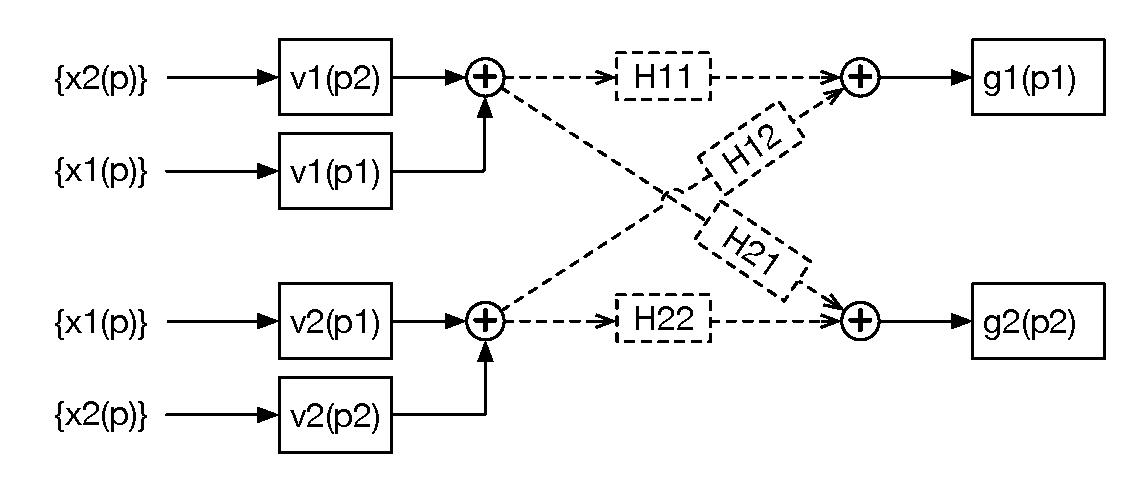
\includegraphics[width=110mm]{forward_channel_2}}
    \caption{Forward Channel}
\end{figure} 

\begin{figure}[h]
    \centering
    \centerline{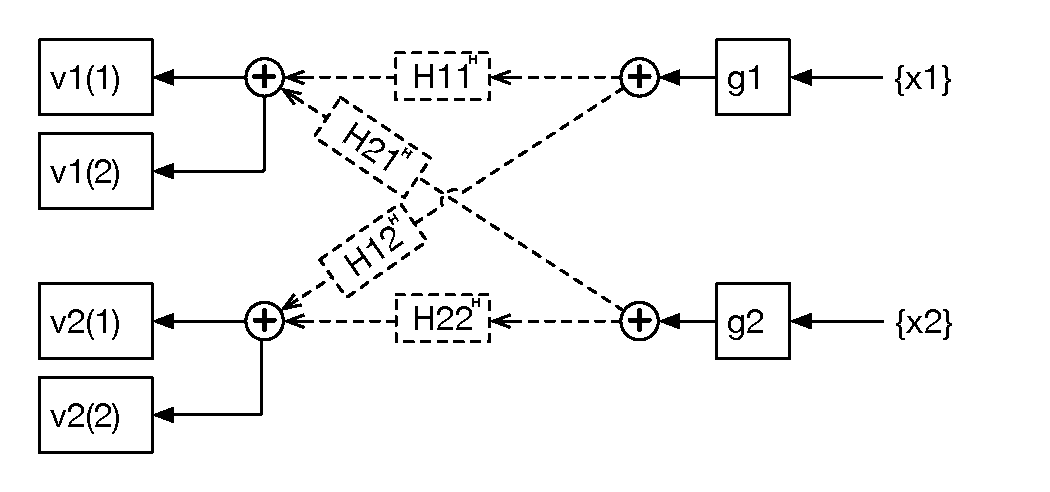
\includegraphics[width=110mm]{backward_channel_2}}
    \caption{Backward Channel}
\end{figure} 

\subsection{Optimization Problem}
\begin{align*}
\min_{\textbf{v}_{k}^{(j)} ,\textbf{g}_{k}} \displaystyle\sum_{k} 	w_k	MSE_{k}	
\end{align*}



\begin{align*}
\text{subject to}  \ \displaystyle\sum_{j}	\|	\textbf{v}^{(j)}_{k}	\|^{2} \leq P; \| \textbf{g}_{k}	\|^{2} \leq P
\end{align*}

where $w_k\in R^{+}$ is weighting factor, and P is the power constraint of transmitters.

\subsection{The received signal vector at k-th receiver}
\begin{align*}
\textbf{y}_{k}  = \displaystyle\sum_{i}		\bigg[	\textbf{H}_{ki}	\displaystyle\sum_{j}	(\textbf{v}^{(j)}_{i}	x_j)		\bigg]	+\textbf{n}_{k}
\end{align*}


\subsection{SINR Derivation}
Our actual objective is to maximize SINR of the system. Since SINR is inversely proportional to MSE, we can simply transform the problem into minimizing MSE of the system.
\begin{align*}
s_{k} = \textbf{g}^{H}_{k}
		(\displaystyle\sum_{i}
		\textbf{H}_{ki} 
		\textbf{v}^{(k)}_{i}x_k)
\end{align*}



\begin{align*}
n_{k} = \textbf{g}^{H}_{k}
		\bigg[\displaystyle\sum_{i}
		\big(	\textbf{H}_{ki} 
		\displaystyle\sum_{j \neq k}	\textbf{v}^{(j)}_{i}x_j	\big)
		+\textbf{n}_{k}\bigg]
\end{align*}

\begin{align*}
\frac	{	|s_{k}|^2	}{	|n_{k}|^2	} = 
\frac {	|\textbf{g}^{H}_{k}
		\displaystyle\sum_{i}
		\textbf{H}_{ki} 
		\textbf{v}^{(k)}_{i}|^2	
	} 
	{	\displaystyle\sum_{j \neq k}
		|\textbf{g}^{H}_{k}
		\displaystyle\sum_{i}
		\textbf{H}_{ki} 
		\textbf{v}^{(j)}_{i}|^2
		+|\textbf{g}^{H}_{k}
		\textbf{R}_{k}
		\textbf{g}_{k}|
	}
\end{align*}

\subsection{Forward Direction}
The solution is simply $R^{-1}p$, where $R$ is the correlation matrix,  and $p$ is the cross-correlation vector.


\begin{align*}
\textbf{g}^*_{k} 	&= \operatornamewithlimits{argmin}_{\textbf{g}_{k}}	(\displaystyle\sum_{k} 	\bigg[	MSE_{k}	+	\lambda_{i}	(\displaystyle\sum_{j}	\|	\textbf{v}^{(j)}_{i}	\|	-P	)	\bigg])	\\
			&= \bigg[	\displaystyle\sum_{j}
				\big[	(\displaystyle\sum_{i}\textbf{H}_{ki}\textbf{v}^{(j)}_{i})
			      (\displaystyle\sum_{i}\textbf{v}^{H(j)}_{i}\textbf{H}^{H}_{ki})	\big]	 +\sigma^2	\textbf{I}
			      \bigg]^{-1}	(\displaystyle\sum_{i}	\textbf{H}_{ki}	\textbf{v}^{(k)}_{i})		      
\end{align*}


\subsection{Backward Direction: Iterative Method which Doesn't Work}

In this method, we found a solution for each $\textbf{v}_{k}^{(j)}$ depending on some $\textbf{v}_{x}^{(j)}$, where k $\neq$ x. For example, $\textbf{v}_{1}^{(1)}$ depends on $\textbf{v}_{2}^{(1)}$. Then, we try to solve the optimization problem by iterating between $\textbf{v}_{k}^{(j)}$ and $\textbf{v}_{x}^{(j)}$, and hope it will work. However, our numerical experiment shows that it will not converge for some channels.
\begin{align*}
MSE_{k} &= \mathrm{E}	[	(	x_k-\textbf{g}^{H}_{k}	\textbf{y}_{k}	)(x_k-\textbf{g}^{H}_{k}	\textbf{y}_{k})^{H}	] \\
		       & = \mathrm{E}[x_k^{2}]	 - \mathrm{E}[x_k	\textbf{y}_{k}^{H} \textbf{g}_{k}]	
		       					-  \mathrm{E}[x_k	\textbf{g}_{k}^{H} \textbf{y}_{k}]
							+ \mathrm{E}[\textbf{g}_{k}^{H} \textbf{y}_{k}	\textbf{y}_{k}^{H} \textbf{g}_{k}]			\\
		       & = 1 - \displaystyle\sum_{i}	\textbf{v}^{H(k)}_{i}	\textbf{H}^{H}_{ki}	\textbf{g}_{k}
		       		- \textbf{g}^{H}_{k}		\displaystyle\sum_{i}	\textbf{H}_{ki}	\textbf{v}^{(k)}_{i}
				+\textbf{g}^{H}_{k}		\displaystyle\sum_{j}
									\bigg[	(\displaystyle\sum_{i}\textbf{H}_{ki}\textbf{v}^{(j)}_{i})
									(\displaystyle\sum_{i}\textbf{v}^{H(j)}_{i}\textbf{H}^{H}_{ki})	\bigg]	\textbf{g}_{k}
				+\sigma^2		\textbf{g}^{H}_{k}	 \textbf{g}_{k}
\end{align*}



\begin{align*}
\textbf{v}^{*(1)}_{1}  &= \operatornamewithlimits{argmin}_{\textbf{v}^{(1)}_{1}}	(\displaystyle\sum_{k=1,2} 	\bigg[	MSE_{k}	+	\lambda_{k}	(\displaystyle\sum_{j=1,2}	\|	\textbf{v}^{(j)}_{k}	\|	-P	)	\bigg])	\\
			       &=\bigg[ 2	\textbf{H}^{H}_{11}	\textbf{g}_{1}	\textbf{g}^{H}_{1}		\textbf{H}_{11}	w_1
				   +	2	\textbf{H}^{H}_{21}	\textbf{g}_{2}	\textbf{g}_{2}		\textbf{H}_{21}	w_2	+2	\lambda^{*}_1 I
				   \bigg]^{-1} 
				   (
				   2	\textbf{H}^{H}_{11}	\textbf{g}_{1}	w_1	
				   -\textbf{g}^{H}_{1}	\textbf{H}_{12}	\textbf{v}^{(1)}_{2} 	\textbf{H}^{H}_{11}	\textbf{g}_{1}	w_1	\\
				   &\ \ \ \ 
				   -	\textbf{H}^{H}_{11}	\textbf{g}_{1}	\textbf{v}^{H(1)}_{2}	\textbf{H}^{H}_{12}	\textbf{g}_{1}	w_1
				   -	\textbf{g}^{H}_{2}	\textbf{H}_{22}	\textbf{v}^{(1)}_{2} 	\textbf{H}^{H}_{21}	\textbf{g}_{2}	w_2
				   -	\textbf{H}^{H}_{21}	\textbf{g}_{2}	\textbf{v}^{H(1)}_{2}	\textbf{H}^{H}_{22}	\textbf{g}_{2}	w_2
				   )\\
			      &=\bigg[	2	\mathrm{E}[x^*_1	\textbf{y}_1]	\mathrm{E}[x^*_1	\textbf{y}_1]^H	w_1
			      			+	2	\mathrm{E}[x^*_2	\textbf{y}_1]	\mathrm{E}[x^*_2	\textbf{y}_1]^H	w_2	+2	\lambda^{*}_1 I
			      	  \bigg]^{-1} 
				  (2	\mathrm{E}[x^*_1	\textbf{y}_1]	w_1
				  -\mathrm{E}[x^*_1	\textbf{y}_2]^H	\textbf{v}^{(1)}_{2} 	\mathrm{E}[x^*_1	\textbf{y}_1]	w_1	\\
				  &\ \ \ \ 	
				  -\mathrm{E}[x^*_1	\textbf{y}_1]	\textbf{v}^{H(1)}_{2} 	\mathrm{E}[x^*_1	\textbf{y}_2]	w_1	
				  -\mathrm{E}[x^*_2	\textbf{y}_2]^H	\textbf{v}^{(1)}_{2} 	\mathrm{E}[x^*_2	\textbf{y}_1]	w_2
				   -\mathrm{E}[x^*_2	\textbf{y}_1]	\textbf{v}^{H(1)}_{2} 	\mathrm{E}[x^*_2	\textbf{y}_2]	w_2	
				   )
\end{align*}







\begin{align*}
\textbf{v}^{*(1)}_{2} 	&= \operatornamewithlimits{argmin}_{\textbf{v}^{(1)}_{2}}	(\displaystyle\sum_{k=1,2} 	\bigg[	MSE_{k}	+	\lambda_{k}	(\displaystyle\sum_{j=1,2}	\|	\textbf{v}^{(j)}_{k}	\|	-P	)	\bigg])	\\
				   &= 	\bigg[ 2	\textbf{H}^{H}_{12}	\textbf{g}_{1}	\textbf{g}^{H}_{1}		\textbf{H}_{12}	w_1
				   +	2	\textbf{H}^{H}_{22}	\textbf{g}_{2}	\textbf{g}^{H}_{2}		\textbf{H}_{22}	w_2	+2	\lambda^{*}_2 I)
				   \bigg]^{-1} 
				   (2	\textbf{H}^{H}_{12}	\textbf{g}_{1}	w_1		
				   -	\textbf{g}^{H}_{1}	\textbf{H}_{11}	\textbf{v}^{(1)}_{1} 	\textbf{H}^{H}_{12}	\textbf{g}_{1} w_1	\\
				   &\ \ \ \ 
				   -	\textbf{H}^{H}_{12}	\textbf{g}_{1}	\textbf{v}^{H(1)}_{1}	\textbf{H}^{H}_{11}	\textbf{g}_{1}	w_1
				   -	\textbf{g}^{H}_{2}	\textbf{H}_{21}	\textbf{v}^{(1)}_{1} 	\textbf{H}^{H}_{22}	\textbf{g}_{2}	w_2
				   -	\textbf{H}^{H}_{22}	\textbf{g}_{2}	\textbf{v}^{H(1)}_{1}	\textbf{H}^{H}_{21}	\textbf{g}_{2}	w_2
				   )\\
				   &=\bigg[	2	\mathrm{E}[x^*_1	\textbf{y}_2]	\mathrm{E}[x^*_1	\textbf{y}_2]^H	w_1
			      			+	2	\mathrm{E}[x^*_2	\textbf{y}_2]	\mathrm{E}[x^*_2	\textbf{y}_2]^H	w_2	+2	\lambda^{*}_2 I
			      	  \bigg]^{-1} 
				  (2	\mathrm{E}[x^*_1	\textbf{y}_2]	w_1
				  -\mathrm{E}[x^*_1	\textbf{y}_1]^H	\textbf{v}^{(1)}_{1} 	\mathrm{E}[x^*_1	\textbf{y}_2]	w_1	\\
				  &\ \ \ \ 	
				  -\mathrm{E}[x^*_1	\textbf{y}_2]	\textbf{v}^{H(1)}_{1} 	\mathrm{E}[x^*_1	\textbf{y}_1]	w_1	
				  -\mathrm{E}[x^*_2	\textbf{y}_1]^H	\textbf{v}^{(1)}_{1} 	\mathrm{E}[x^*_2	\textbf{y}_2]	w_2
				   -\mathrm{E}[x^*_2	\textbf{y}_2]	\textbf{v}^{H(1)}_{1} 	\mathrm{E}[x^*_2	\textbf{y}_2]	w_2	
				   )
\end{align*}


\begin{align*}
\textbf{v}^{*(2)}_{1}  &= \operatornamewithlimits{argmin}_{\textbf{v}^{(2)}_{1}}	(\displaystyle\sum_{k=1,2} 	\bigg[	MSE_{k}	+	\lambda_{k}	(\displaystyle\sum_{j=1,2}	\|	\textbf{v}^{(j)}_{k}	\|	-P	)	\bigg])	\\
			       &=\bigg[ 2	\textbf{H}^{H}_{11}	\textbf{g}_{1}	\textbf{g}^{H}_{1}		\textbf{H}_{11}	w_1
				   +	2	\textbf{H}^{H}_{21}	\textbf{g}_{2}	\textbf{g}_{2}		\textbf{H}_{21}	w_2	+2	\lambda^{*}_1 I
				   \bigg]^{-1} 
				   (
				   2	\textbf{H}^{H}_{21}	\textbf{g}_{2}	w_2	
				   -\textbf{g}^{H}_{1}	\textbf{H}_{12}	\textbf{v}^{(2)}_{2} 	\textbf{H}^{H}_{11}	\textbf{g}_{1}	w_1	\\
				   &\ \ \ \ 
				   -	\textbf{H}^{H}_{11}	\textbf{g}_{1}	\textbf{v}^{H(2)}_{2}	\textbf{H}^{H}_{12}	\textbf{g}_{1}	w_1
				   -	\textbf{g}^{H}_{2}	\textbf{H}_{22}	\textbf{v}^{(2)}_{2} 	\textbf{H}^{H}_{21}	\textbf{g}_{2}	w_2
				   -	\textbf{H}^{H}_{21}	\textbf{g}_{2}	\textbf{v}^{H(2)}_{2}	\textbf{H}^{H}_{22}	\textbf{g}_{2}	w_2
				   )\\
			      &=\bigg[	2	\mathrm{E}[x^*_1	\textbf{y}_1]	\mathrm{E}[x^*_1	\textbf{y}_1]^H	w_1
			      			+	2	\mathrm{E}[x^*_2	\textbf{y}_1]	\mathrm{E}[x^*_2	\textbf{y}_1]^H	w_2	+2	\lambda^{*}_1 I
			      	  \bigg]^{-1} 
				  (2	\mathrm{E}[x^*_2	\textbf{y}_1]	w_2
				  -\mathrm{E}[x^*_1	\textbf{y}_2]^H	\textbf{v}^{(2)}_{2} 	\mathrm{E}[x^*_1	\textbf{y}_1]	w_1	\\
				  &\ \ \ \ 	
				  -\mathrm{E}[x^*_1	\textbf{y}_1]	\textbf{v}^{H(2)}_{2} 	\mathrm{E}[x^*_1	\textbf{y}_2]	w_1	
				  -\mathrm{E}[x^*_2	\textbf{y}_2]^H	\textbf{v}^{(2)}_{2} 	\mathrm{E}[x^*_2	\textbf{y}_1]	w_2
				   -\mathrm{E}[x^*_2	\textbf{y}_1]	\textbf{v}^{H(2)}_{2} 	\mathrm{E}[x^*_2	\textbf{y}_2]	w_2	
				   )
\end{align*}


\begin{align*}
\textbf{v}^{*(2)}_{2} 	&= \operatornamewithlimits{argmin}_{\textbf{v}^{(2)}_{2}}	(\displaystyle\sum_{k=1,2} 	\bigg[	MSE_{k}	+	\lambda_{k}	(\displaystyle\sum_{j=1,2}	\|	\textbf{v}^{(j)}_{k}	\|	-P	)	\bigg])	\\
				   &= 	\bigg[ 2	\textbf{H}^{H}_{12}	\textbf{g}_{1}	\textbf{g}^{H}_{1}		\textbf{H}_{12}	w_1
				   +	2	\textbf{H}^{H}_{22}	\textbf{g}_{2}	\textbf{g}^{H}_{2}		\textbf{H}_{22}	w_2	+2	\lambda^{*}_2 I)
				   \bigg]^{-1} 
				   (2	\textbf{H}^{H}_{22}	\textbf{g}_{2}	w_2		
				   -	\textbf{g}^{H}_{1}	\textbf{H}_{11}	\textbf{v}^{(2)}_{1} 	\textbf{H}^{H}_{12}	\textbf{g}_{1} w_1	\\
				   &\ \ \ \ 
				   -	\textbf{H}^{H}_{12}	\textbf{g}_{1}	\textbf{v}^{H(2)}_{1}	\textbf{H}^{H}_{11}	\textbf{g}_{1}	w_1
				   -	\textbf{g}^{H}_{2}	\textbf{H}_{21}	\textbf{v}^{(2)}_{1} 	\textbf{H}^{H}_{22}	\textbf{g}_{2}	w_2
				   -	\textbf{H}^{H}_{22}	\textbf{g}_{2}	\textbf{v}^{H(2)}_{1}	\textbf{H}^{H}_{21}	\textbf{g}_{2}	w_2
				   )\\
				   &=\bigg[	2	\mathrm{E}[x^*_1	\textbf{y}_2]	\mathrm{E}[x^*_1	\textbf{y}_2]^H	w_1
			      			+	2	\mathrm{E}[x^*_2	\textbf{y}_2]	\mathrm{E}[x^*_2	\textbf{y}_2]^H	w_2	+2	\lambda^{*}_2 I
			      	  \bigg]^{-1} 
				  (2	\mathrm{E}[x^*_2	\textbf{y}_2]	w_2
				  -\mathrm{E}[x^*_1	\textbf{y}_1]^H	\textbf{v}^{(2)}_{1} 	\mathrm{E}[x^*_1	\textbf{y}_2]	w_1	\\
				  &\ \ \ \ 	
				  -\mathrm{E}[x^*_1	\textbf{y}_2]^H	\textbf{v}^{H(2)}_{1} 	\mathrm{E}[x^*_1	\textbf{y}_1]	w_1	
				  -\mathrm{E}[x^*_2	\textbf{y}_1]^H	\textbf{v}^{(2)}_{1} 	\mathrm{E}[x^*_2	\textbf{y}_2]	w_2
				   -\mathrm{E}[x^*_2	\textbf{y}_2]^H	\textbf{v}^{H(2)}_{1} 	\mathrm{E}[x^*_2	\textbf{y}_1]	w_2	
				   )
\end{align*}




\subsection{Backward Direction: Duality Method}
For the duality method, if the optimization problem is convex, then the optimal solution is guaranteed. If it is not, there will exist a \textbf{duality gap} which will not give the optimal solution[Convex Optimization, Boyd]. Since our problem is non-convex, getting the optimal solution is possible but not guaranteed. The same problem with single constraint(only contains one $\lambda$) has been solved[Boyd], but not for the cases with multiple constraints. \textbf{However, our numerical result shows that there's no duality gap, which means we actually get the optimal solution!}

\subsubsection{Convexity Analysis}

We could rewrite our cost function in
\begin{align*}
\displaystyle\sum_{k} 	w_k	MSE_{k}	=  (\displaystyle\sum_{k} w_k)-\textbf{kv}-(\textbf{kv})^{H}+\textbf{v}^{H}\textbf{A}\textbf{v}+ \sigma^{2} \textbf{g}^{H} \textbf{g}
\end{align*}

where \textbf{k} is a constant row vector with channel information, \textbf{A} is a constant matrix with channel information, and $\pmb{\lambda}$ is a diagonal matrix with each $\pmb{\lambda}_{ii}$ to be some $\lambda_{k}$. Since A is \textbf{not a positive definite} matrix, the cost function is non-convex. In addition, \textbf{A} has very similar properties to the \textbf{correlation matrix} in adaptive filter theory. Due to no additional noise on transmitter side, \textbf{A} is singular.




\subsubsection{Primal Problem}
It's the same as the optimization problem in 2.1. 

\subsubsection{Primal Algorithm}
\begin{align*}
\min_{\textbf{v}_{k}^{(j)}}\
L( \textbf{v}, \pmb{\lambda} )=\displaystyle\sum_{k} 	\bigg[w_k	MSE_{k}	+	\lambda_{k}	(\displaystyle\sum_{j}	\|	\textbf{v}^{(j)}_{k}	\|	-P	)	\bigg]
\end{align*}
Since the Lagrangian L is \textbf{not always convex(depends on $\lambda_{k}$)}, using gradient descent can only give \textbf{local optimum}. There do exist better ways to deal with non-convex problems, with potential to find global optimum, such as  \textbf{line search with Wolfe condition}. However, due to the enormous complexity of Wolfe algorithm, we choose to stay with gradient descent. The gradient is

\begin{align*}
\frac{\partial L( \textbf{v}, \pmb{\lambda} )}{\partial \textbf{v}} = -2\textbf{k}+2\textbf{v}^{H}[\textbf{A}+\pmb{\lambda}]
\end{align*}

and the algorithm is
\begin{align*}
\textbf{v}(i+1) = \textbf{v}(i) - \mu_\textbf{v} (\frac{\partial L( \textbf{v}, \pmb{\lambda} )}{\partial \textbf{v}})^{H}
\end{align*}

where $\mu_\textbf{v}$ is a fixed stepsize.







\subsubsection{Dual Problem}

\begin{align*}
\max_{	\pmb{\lambda} \geq \textbf{0}	}	G( \textbf{v}^{*}, \pmb{\lambda} ) \ = 
\max_{	\pmb{\lambda}	\geq \textbf{0}}
[
\min_{\textbf{v}_{k}^{(j)}}\
L( \textbf{v}, \pmb{\lambda} )]
\end{align*}

The \textbf{feasible set} of $\lambda_{k}$ is positive number set. The reason could be found in textbook. 

\subsubsection{Dual Algorithm}

By the optimization theory, dual problems are \textbf{always} concave. Therefore, we could get the optimal $\pmb{\lambda}$ simply with gradient algorithm. The gradient is shown below.


\begin{align*}
\frac{\partial G( \textbf{v}^{*}, \pmb{\lambda} )}{\partial \lambda_{k}} = 
\displaystyle\sum_{j}	\|	\textbf{v}^{(j)}_{k}	\|	-P
\end{align*}

The algorithm is 

\begin{align*}
 \pmb{\lambda} (i+1) =  \pmb{\lambda}(i) + \mu_{\pmb{\lambda}} (\frac{\partial L( \textbf{v}^{*}, \pmb{\lambda} )}{\partial \ \pmb{\lambda}})^{T},  \pmb{\lambda}	\geq \textbf{0}
\end{align*}

where $\mu_{\pmb{\lambda}}$ is a fixed stepsize.





\subsection{Backward Direction: Noisy Transmitter Approach}

In the duality method section, we've seen that our cost function is non-convex. However, in practical situation, there must exist some noise at transmitters. Thus, with the presence of noise, the system becomes convex. With this assumption, we could get the analytical solution for this problem. 
We get 
\begin{align*}
\textbf{v}^{*H} = \textbf{k}[\textbf{A}+\pmb{\lambda}]^{-1}, \forall \lambda_{k} \geq 0
\end{align*}
The corresponding dual problem is

\begin{align*}
\max_{	\pmb{\lambda} \geq \textbf{0}	}	G( \textbf{v}^{*}, \pmb{\lambda} ) \ = 
\max_{	\pmb{\lambda}	\geq \textbf{0}}
[
\min_{\textbf{v}_{k}^{(j)}}\
L( \textbf{v}, \pmb{\lambda} )]=
\max_{	\pmb{\lambda}	\geq \textbf{0}}\ \displaystyle\sum_{k} (w1+w2+w3) - \textbf{v}^{*H}\textbf{k}^{H} + \sigma^{2} \textbf{g}^{H} \textbf{g} - P(\lambda_{1}+\lambda_{2}+\lambda_{3})
\end{align*}


We could actually find the \textbf{analytic solution} for $\pmb{\lambda}$. However, for 3 users case, the process includes finding the \textbf{inverse of an 6x6 symbolic matrix}  which is \textbf{solvable} but \textbf{complicated}, let alone cases above 3 users. Thus, we choose to solve the dual problem with \textbf{numerical method}. By the optimization theory, dual problems are \textbf{always} convex. Therefore, we could get the optimal $\pmb{\lambda}$ simply with gradient algorithm. The gradient is shown below.

\begin{align*}
\frac{\partial G( \textbf{v}^{*}, \pmb{\lambda} )}{\partial \lambda_{k}} = 
-P+
\Tr[
(A+\pmb{\lambda})^{-T}\textbf{k}^{H}\textbf{k}(A+\pmb{\lambda})^{-T}
]
\end{align*}




\subsection{Turning into Bi-Directional Training}
There will be some issues if we want to transform the optimization problem into bi-directional training algorithm. First, \textbf{the algorithm we provided doesn't really solve the optimization problem.} The reason is that we deal the variables $\textbf{v}$ and $\textbf{g}$ separately. In order to get the optimizer of this problem, we need to find the optimizer over a single variable [$\textbf{v}$,$\textbf{g}$]. \textbf{The second issue is about the power constraint of $\textbf{g}$}. For $\textbf{v}$, the magnitude is controlled by the lagrange multiplier $\lambda$. However, for $\textbf{g}$, we don't have such mechanism. Thus, we adopt the following \textbf{scaling method}: 
\[
  \textbf{g}_k = \left\{\def\arraystretch{1.2}%
  \begin{array}{@{}c@{\quad}l@{}}
    \textbf{g}_k  & \text{if $\| \textbf{g}_k \|^{2} \leq P$}\\
    \frac{\sqrt{P}}{\| \textbf{g}_k \|} \textbf{g}_k& \text{if $\| \textbf{g}_k \|^{2} > P$}\\
  \end{array}\right.
\]

\subsection{Numerical Results}
For numerical simulation, we compare the performance of 3 different algorithms/models. By simple transmitter, we mean system model in [Shi, 2014]. The diagram of the simple transmitter is also shown below. First thing to notice is \textbf{we set some of the power constraints to be $\leq P$ or $= P$}. The reason behind this is there really is \textbf{no noticeable difference in numerical results}(I've done both of them). The second thing is that we can only guarantee that method 1 will perform best. The reason why method 2 may not be better than method 3 is simple: Transmitters in method 2 cannot cooperate with each other, which may produce additional interference. 

 \begin{figure}[h]
    \centering
    \centerline{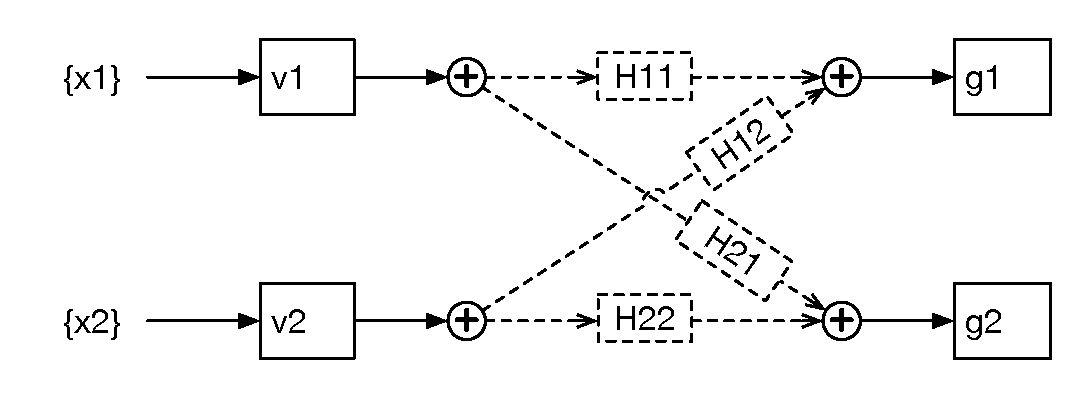
\includegraphics[width=110mm]{forward_channel_4}}
    \caption{Simple Transmitters}
\end{figure} 



\begin{table}[h!]
\centering
\begin{tabular}{ |p{3cm}||p{3cm}|p{3cm}|p{3cm}|  }
 \hline
& Coop.(Duality) &Coop.($R^{-1}p$)&Simple\\
 \hline
 System Model   & 2   &2&   Simple\\
 Forward Alg.      &  $R^{-1}p$  & $R^{-1}p$ &$R^{-1}p$\\
 Backward Alg.   &Duality & $R^{-1}p$&  $R^{-1}p$\\ 
 g constraint      &$\leq P$& $\leq P$\ or\ $= P$&  $\leq P$\ or\ $= P$\\ 
 v constraint       &$\leq P$ & \ $= P$& \ $= P$\\ 
 \hline
\end{tabular}
\caption{3 different algorithms/models}
\end{table}


\newpage


\subsubsection{Sum Capacity vs. Iterations}
\textbf{A. Iteration Count:} Start with backward training. A full cycle of backward then forward training counts as 1 iteration.
\newline
\textbf{B. Parameters:}
\newline
1. Number of User $k$ = 3
\newline
2. Power Constraint $P$ = 1
\newline
3. Noise Variance $n_0$=$\mathbb{E}[\textbf{n}_k^{H}\textbf{n}_k]$ ranges from $10^{-3}$ to $10^{-1}$
\newline
4. Results are averaged over 100 random complex gaussian channels.
\newline
5. Channel Capacity $C = \log_2 ({1+SINR})$


\begin{figure}[H]
    \centering
    \centerline{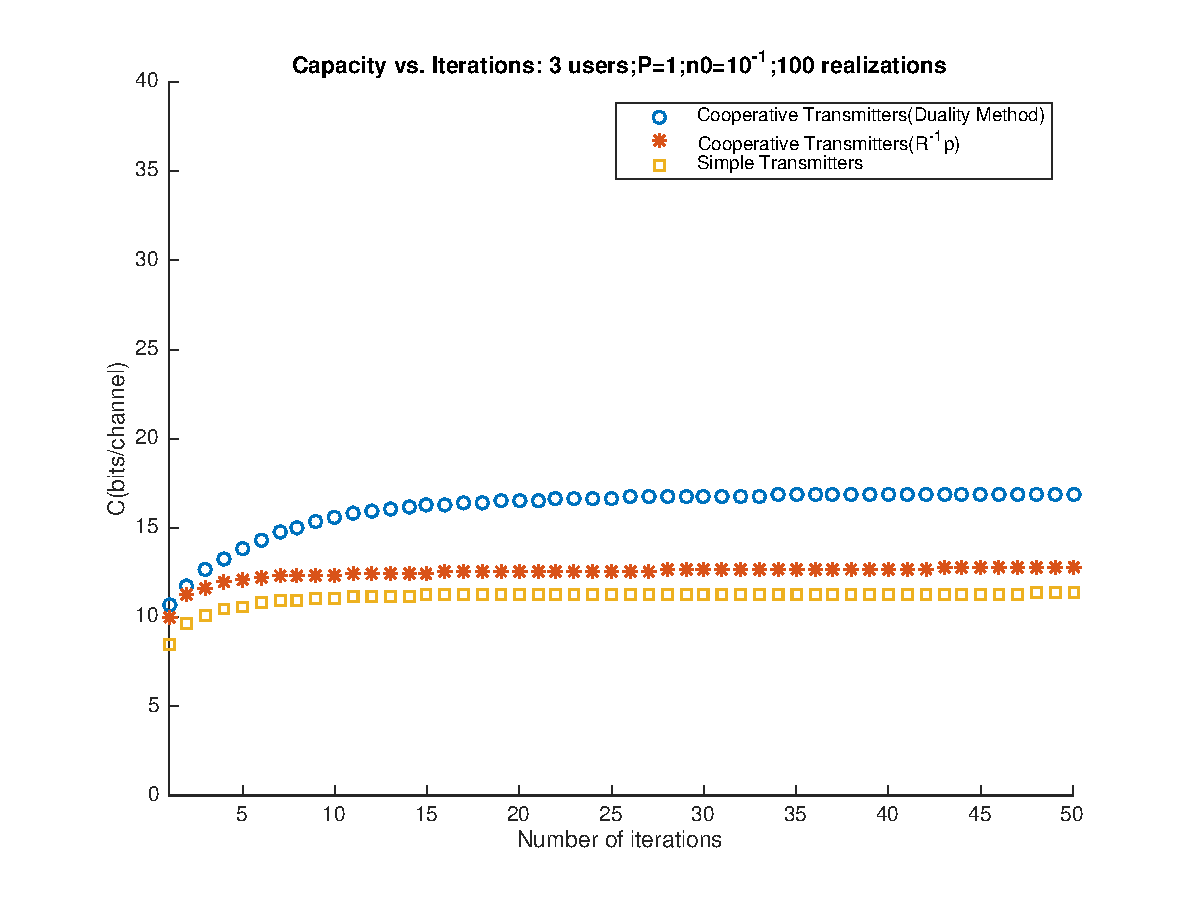
\includegraphics[width=110mm]{4}}
    \caption{Noise Variance $n0=10^{-1}$}
\end{figure} 

\begin{figure}[H]
    \centering
    \centerline{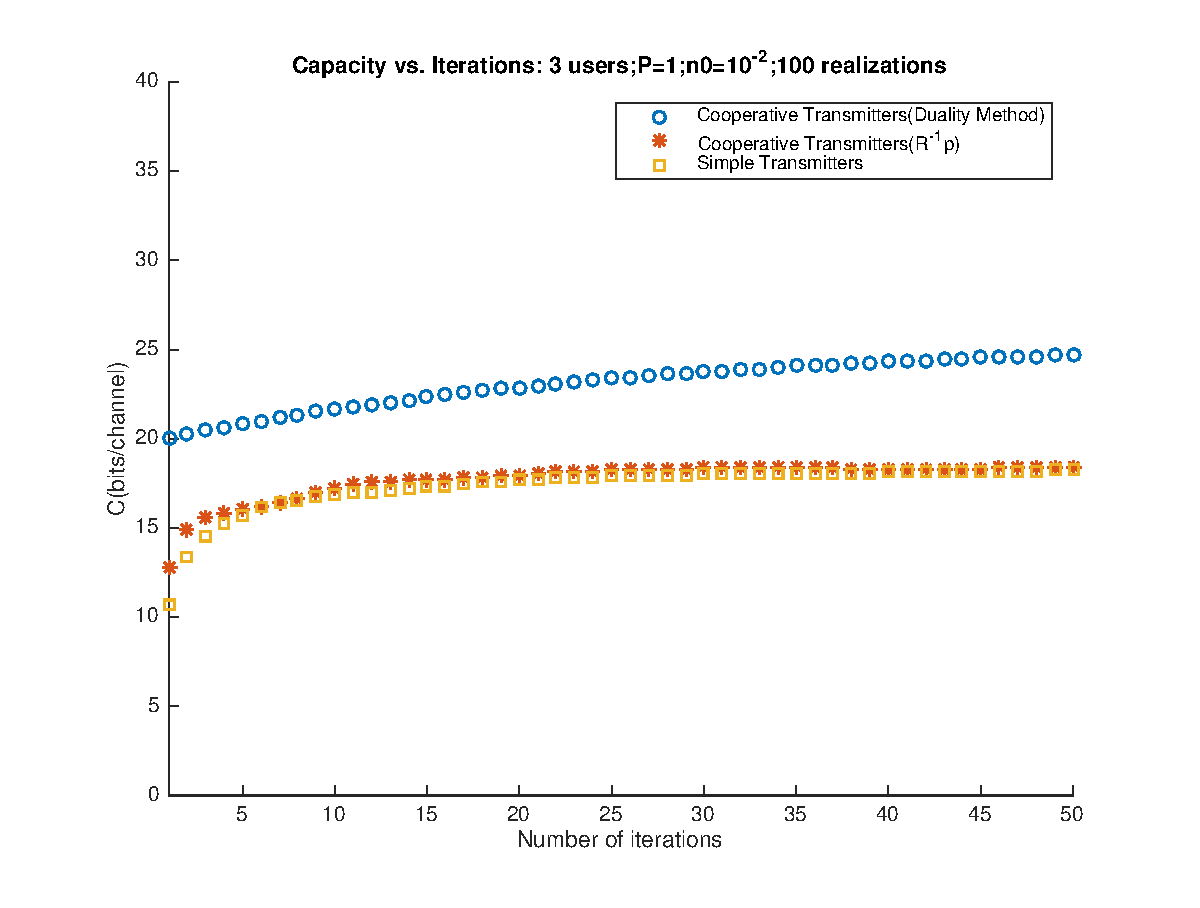
\includegraphics[width=110mm]{5}}
    \caption{Noise Variance $n0=10^{-2}$}
\end{figure} 

\begin{figure}[H]
    \centering
    \centerline{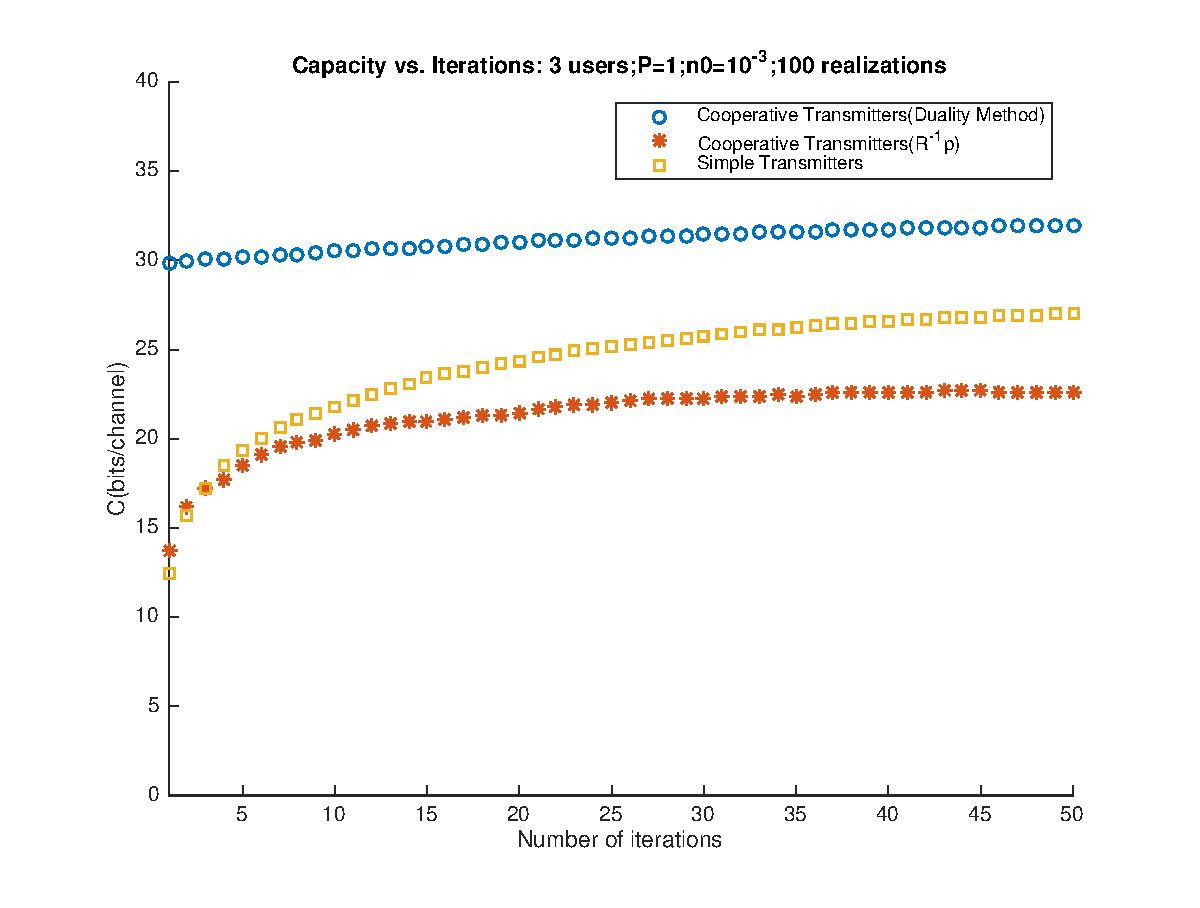
\includegraphics[width=110mm]{6}}
    \caption{Noise Variance $n0=10^{-3}$}
\end{figure} 

\subsubsection{Sum Capacity vs. Noise}
\textbf{A. Convergence Criterion:} As we can see from the previous example, filters tend to converge at \textbf{20th iteration}. Thus, we choose 20 iterations for doing this simulation.
\newline
\textbf{B. Parameters:}
\newline
1. Number of User $k$ = 3
\newline
2. Power Constraint $P$ = 1
\newline
3. Noise Variance $n_0$=$\mathbb{E}[\textbf{n}_k^{H}\textbf{n}_k]$ ranges from $10^{-3}$ to $1$
\newline
4. Results are averaged over 10 random complex gaussian channels.
\newline
5. Channel Capacity $C = \log_2 ({1+SINR})$


\newpage

\section{System Model 3 : Augmented Receivers}
In this model, we make each receivers(mobile station) possess the ability to assist channel estimation in backward direction. Since it is rather easy to add a filter to receivers, if this method does improve the capacity, it will be extremely fascinating. We solve each transceivers with Wiener-Hopf equation: $R^{-1}p$.

 \begin{figure}[h]
    \centering
    \centerline{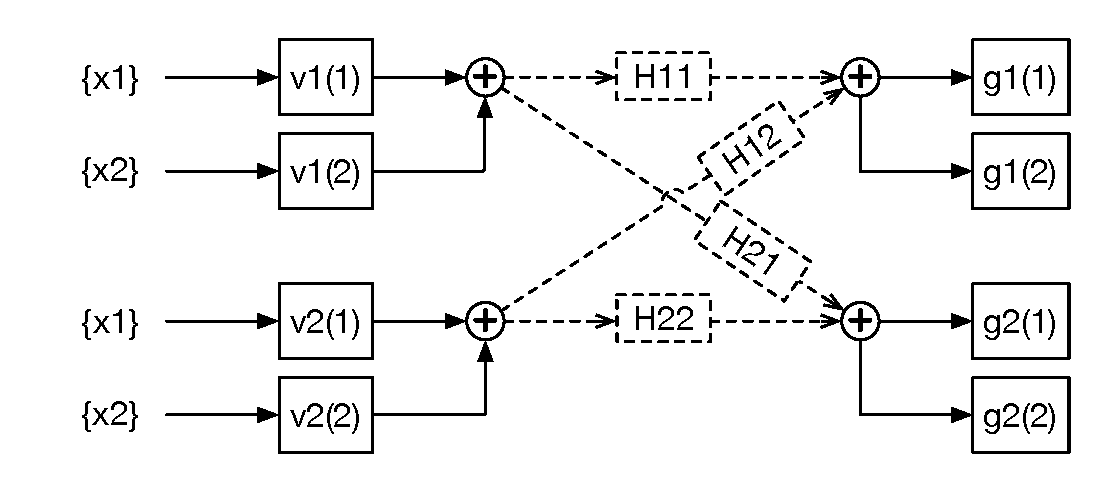
\includegraphics[width=110mm]{forward_channel_3}}
    \caption{Forward Channel}
\end{figure} 

\begin{figure}[h]
    \centering
    \centerline{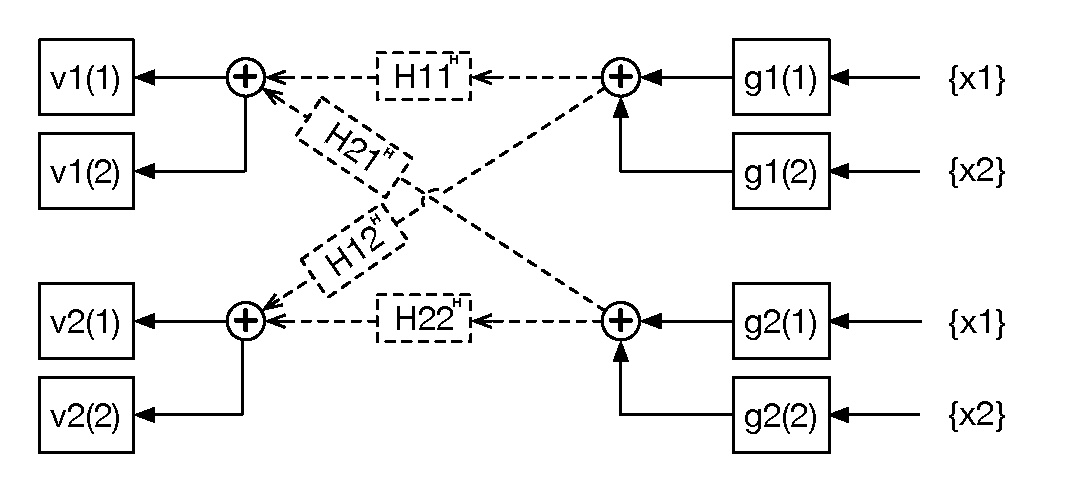
\includegraphics[width=110mm]{backward_channel_3}}
    \caption{Backward Channel}
\end{figure} 

\subsection{Optimization Problem}
\begin{align*}
\min_{\textbf{v}_{k}^{(j)} ,\textbf{g}_{k}} \displaystyle\sum_{k} 	w_k	MSE_{k}	
\end{align*}

\begin{align*}
\text{subject to}  \ \displaystyle\sum_{j}	\|	\textbf{v}^{(j)}_{k}	\|^{2} = P; \| \textbf{g}_{k}	\|^{2} = P
\end{align*}


\subsection{Numerical Results}
This is a 3 users, and 2X2 MIMO interference channel, with SNR equals to 20dB. The results are averaged over 1000 complex gaussian channels. X-axis represents the number of iterations: start from backward direction and end in forward direction. Y-axis represents the sum capacity of three users. The first thing we can tell is the \textbf{augmented one} is a lot worse than the \textbf{simple one}(Only one filter at each transceivers. For example, for 2 users case, only have $v^{(1)}_1$,$v^{(2)}_2$,$g^{(1)}_1$,$g^{(2)}_2$ ). \textbf{This is because transmitters distribute all messages to all users.} In the experiment, transmitter 1 sends 2 bits of message 1 to user 1, 2, and 3. However user 2 and 3 simply drop message 1 off(they don't need it). Thus, the sum capacity of augmented receivers only have 1/3 of capacity compared with the simple one.

 \begin{figure}[h]
    \centering
    \centerline{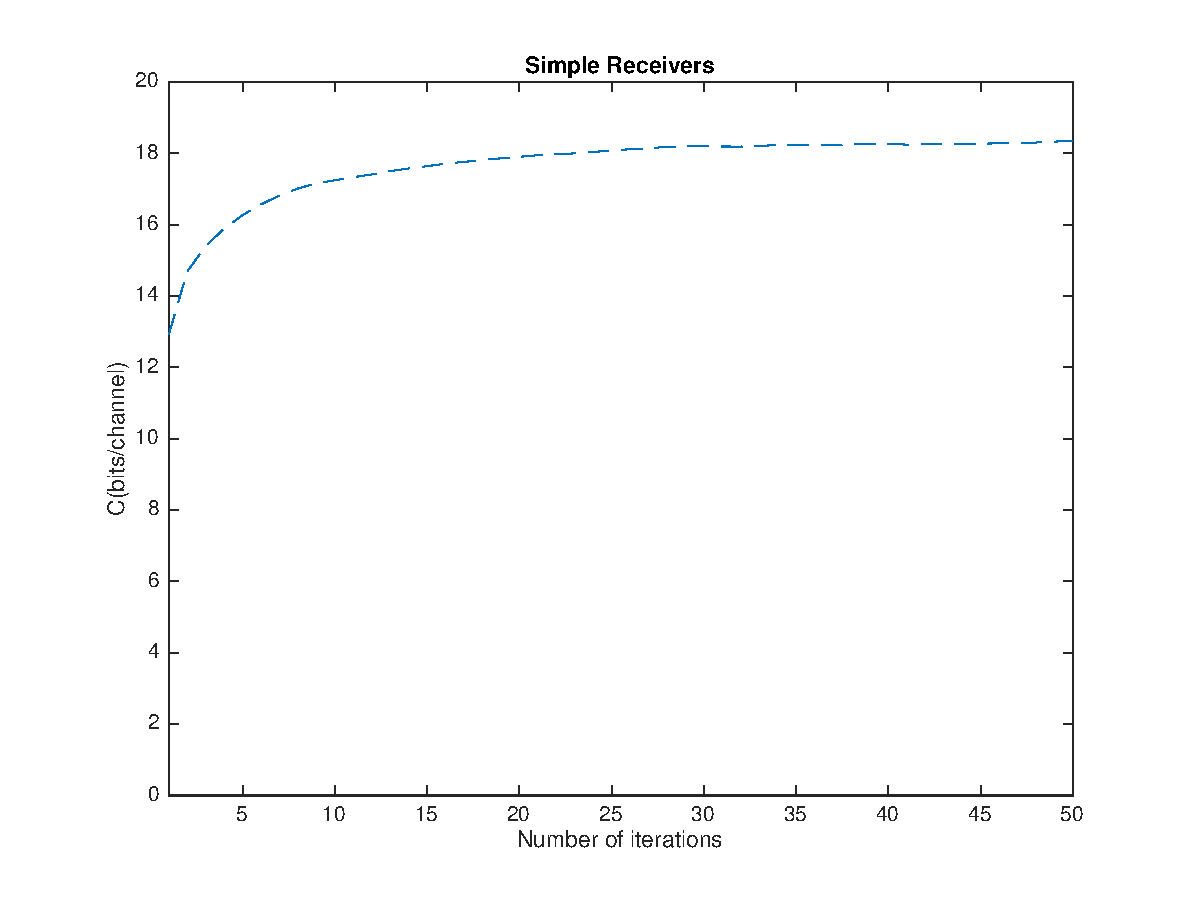
\includegraphics[width=110mm]{Simple_Receivers}}
    \caption{Simple Receivers}
\end{figure} 

\begin{figure}[h]
    \centering
    \centerline{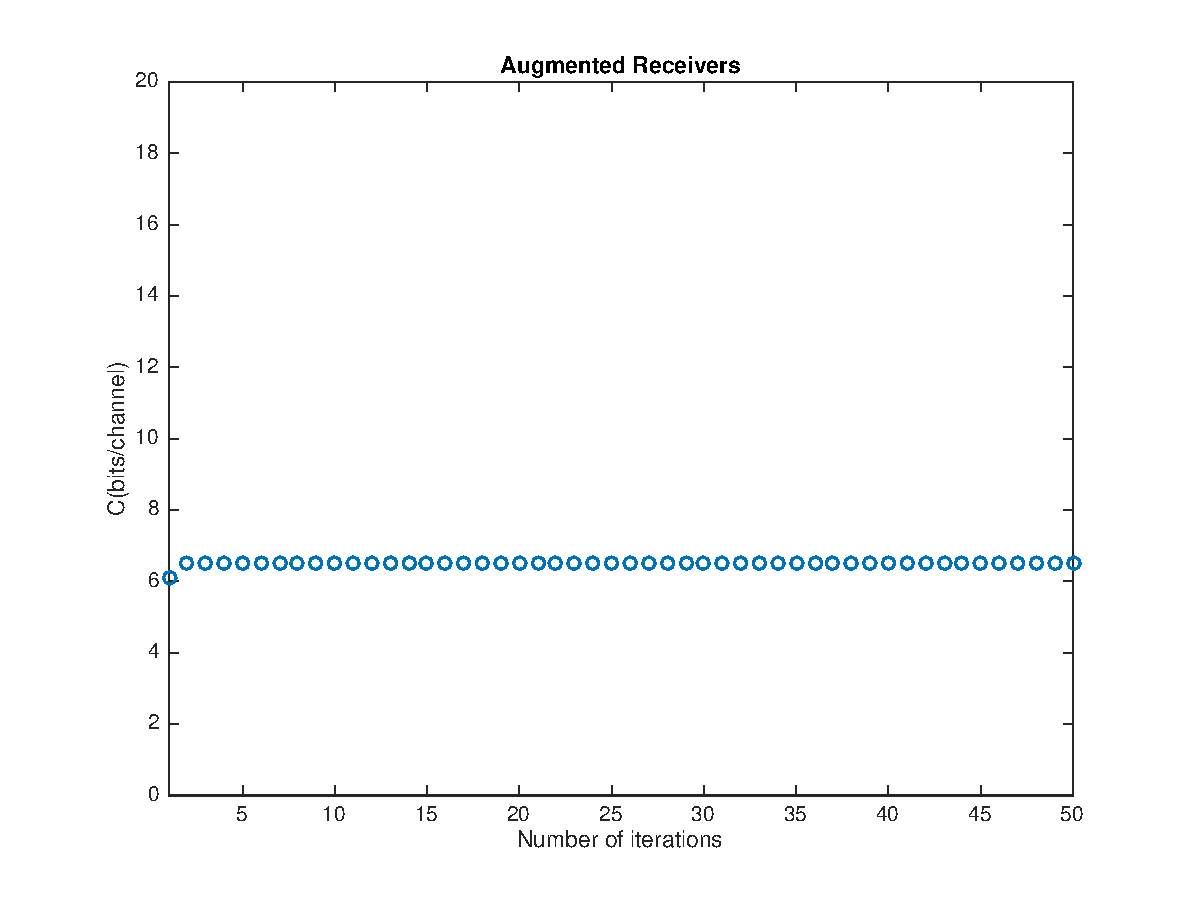
\includegraphics[width=110mm]{Augmented_Receivers}}
    \caption{Augmented Receivers}
\end{figure} 





\newpage
There's an interesting result of $\lambda_{k}$. This is, if we \textbf{change our constraint from equality to inequality}, the duality method will give the same answer. Although this is not too surprising, it is justified by mathematics.
9. Numerical Simulation(2 Users, 2X2 MIMO Channel)


\begin{align*}
Rayleigh\ Fading\ Channel
\end{align*}

\begin{align*}
\ Cross\ Channel\ Gain = 0.8*Direct\ Channel\ Gain
\end{align*}

\begin{align*}
SNR = \frac {1}{\sigma^2} = 10^3=30dB
\end{align*}

\begin{align*}
Observation1: &If\ the\ training\ length\ is\ long\ enough,\ each\ LMS\ filter\ (\textbf{v}^{(c)}_{k},\textbf{v}^{(p)}_{k},\textbf{g}^{(c)}_{k},\textbf{g}^{(p)}_{k},)\\
&will\ converge\ to\ Wiener\ filter
\end{align*}

\begin{align*}
Observation2:\ Use\ Wiener\ filters,\ and\ only\ send\ common\ messages.\ Sum\ rate\ C\ =\ 11.6\ bit/channel
\end{align*}

\begin{align*}
Observation3:\ Use\ Wiener\ filters,\ and\ only\ send\ private\ messages.\ Sum\ rate\ C\ =\ 2.63\ bit/channel
\end{align*}

\begin{align*}
Observation4:\ Use\ Wiener\ filters,\ and\  send\ both\ messages.\ Sum\ rate\ C\ =\ 3.35\ bit/channel
\end{align*}

\begin{align*}
Observation5:\ Under\ the\ cooperation\ scheme,\ transmitters\ don't\ converge\ to\ Wiener\ filters 
\end{align*}

\begin{align*}
Observation5:\ Under\ the\ cooperation\ scheme,\ C=3.15\ bit/channel
\end{align*}



\begin{figure}[bp!]
    \centering
    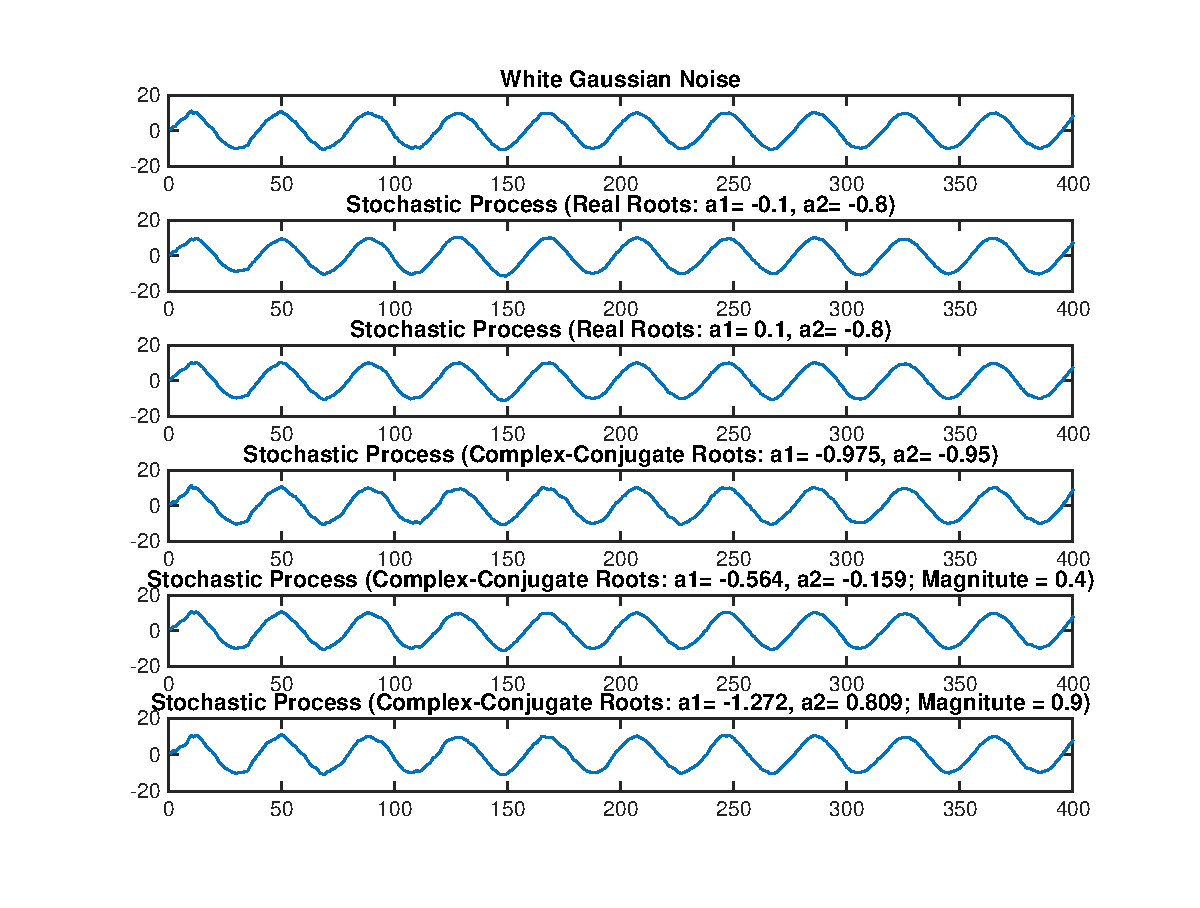
\includegraphics[width=150mm]{01}
    \caption{Insert caption}
\end{figure} 

\begin{figure}[bp!]
    \centering
    \centerline{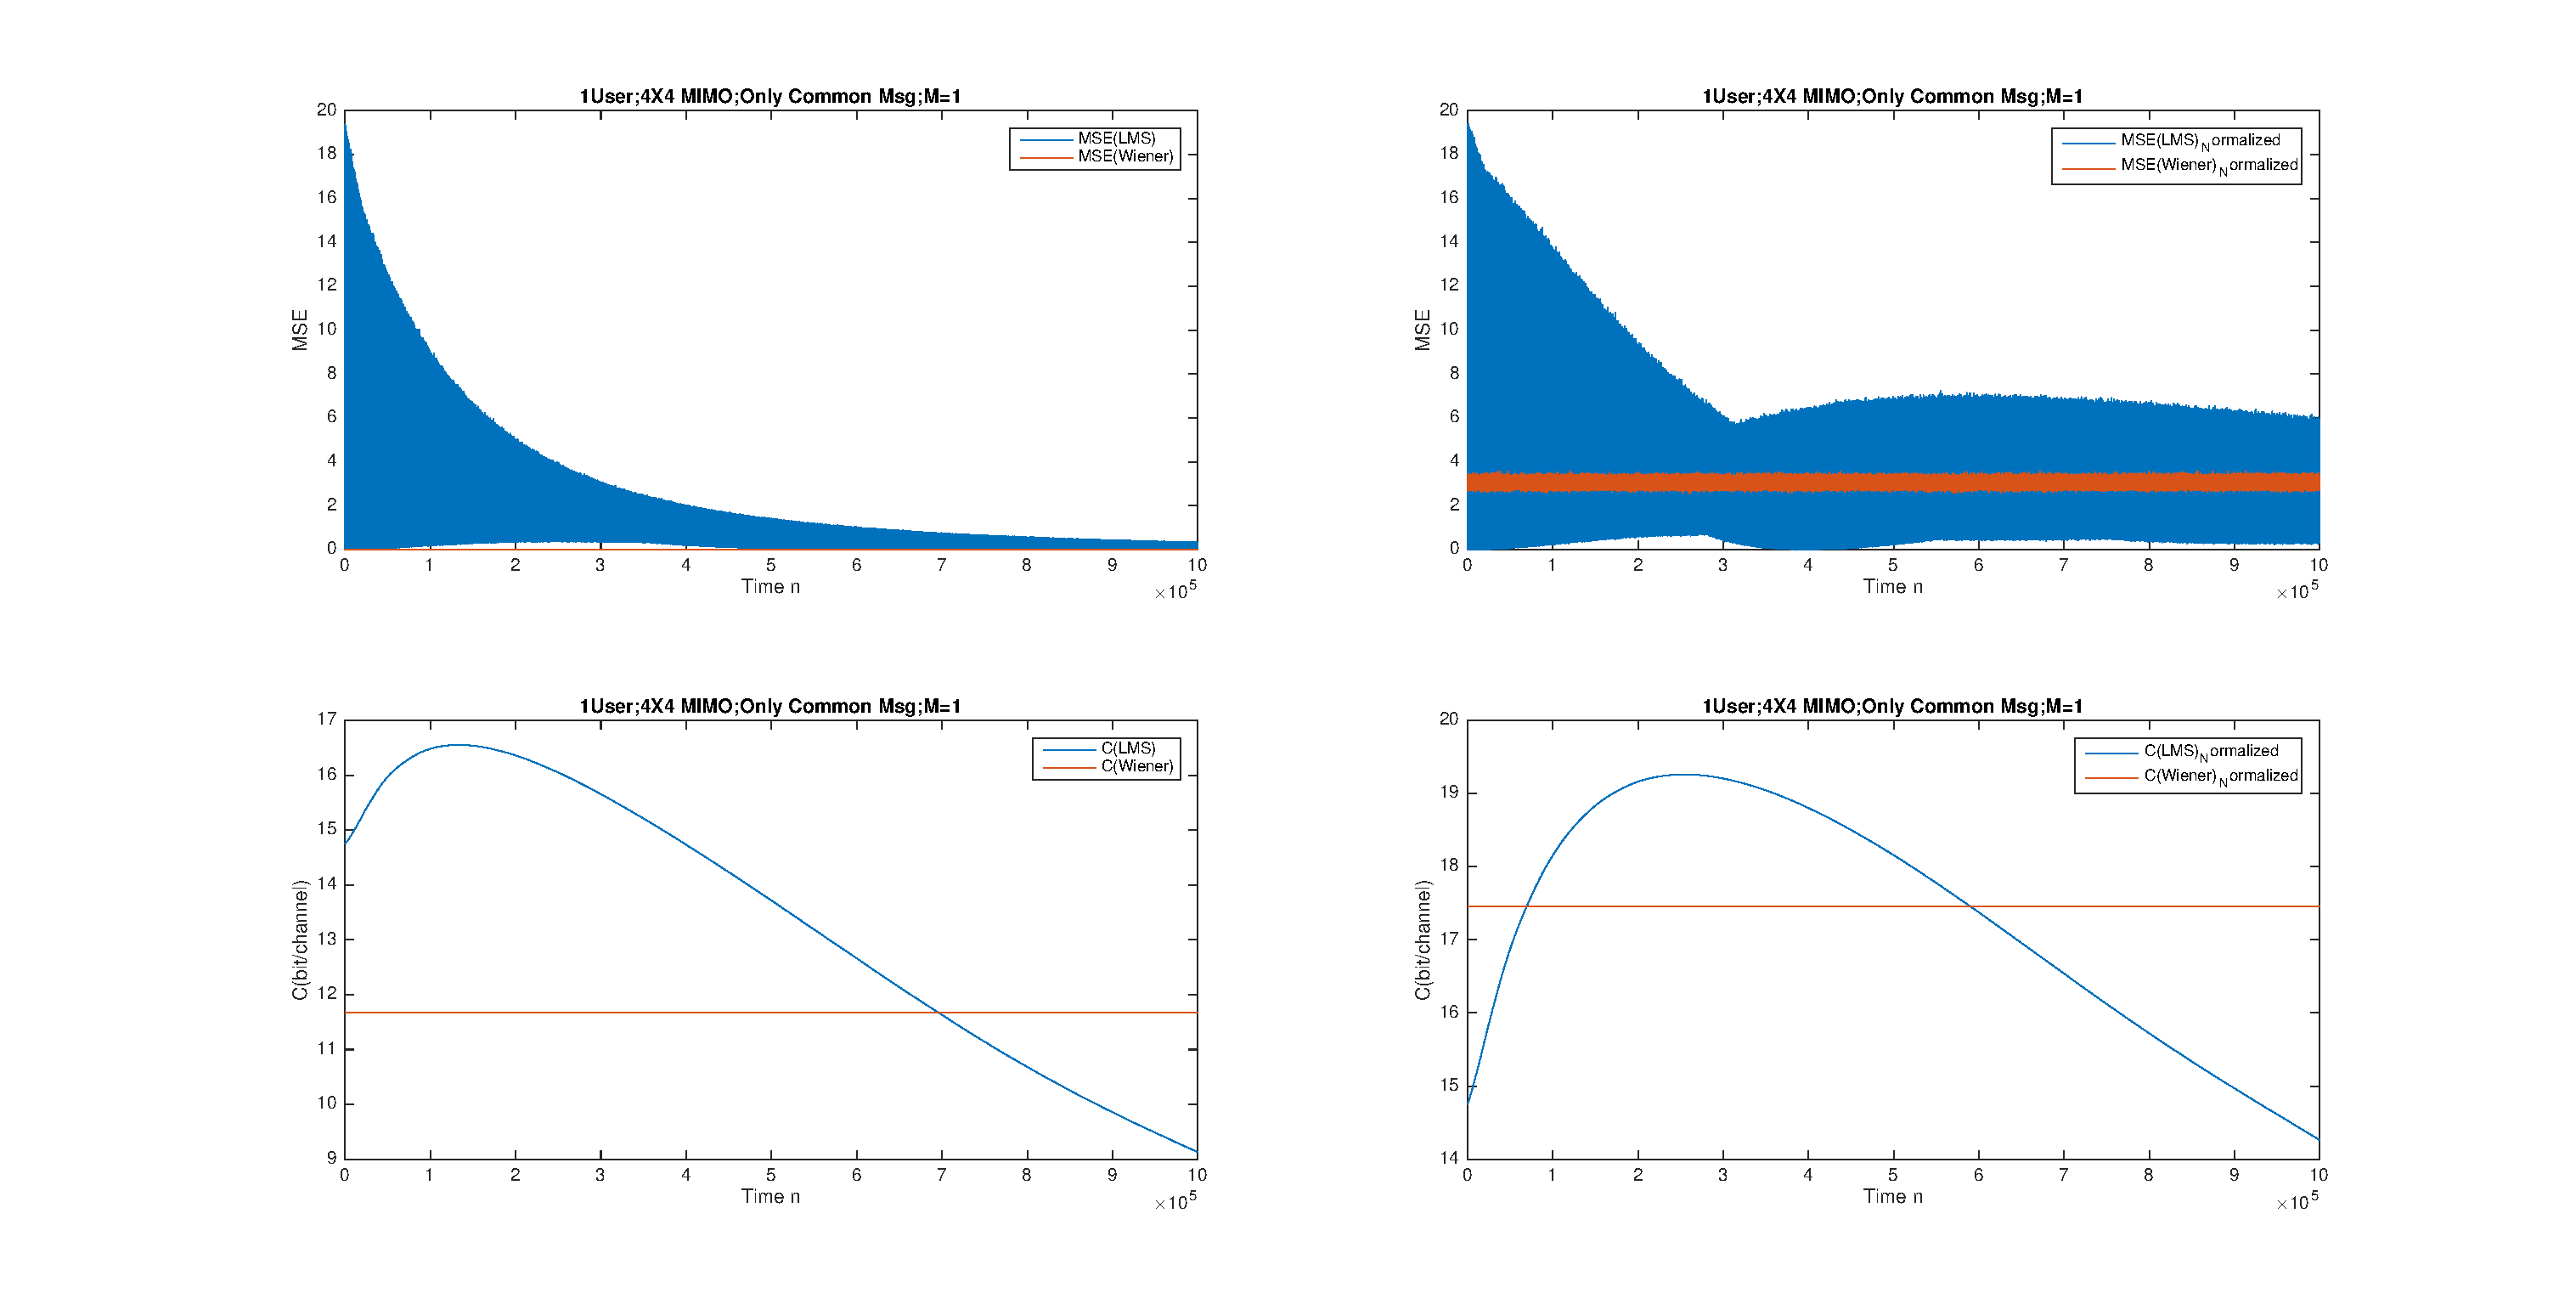
\includegraphics[width=220mm]{1USER_4X4MIMO}}
    \caption{Insert caption}
\end{figure} 

\begin{figure}[bp!]
    \centering
    \centerline{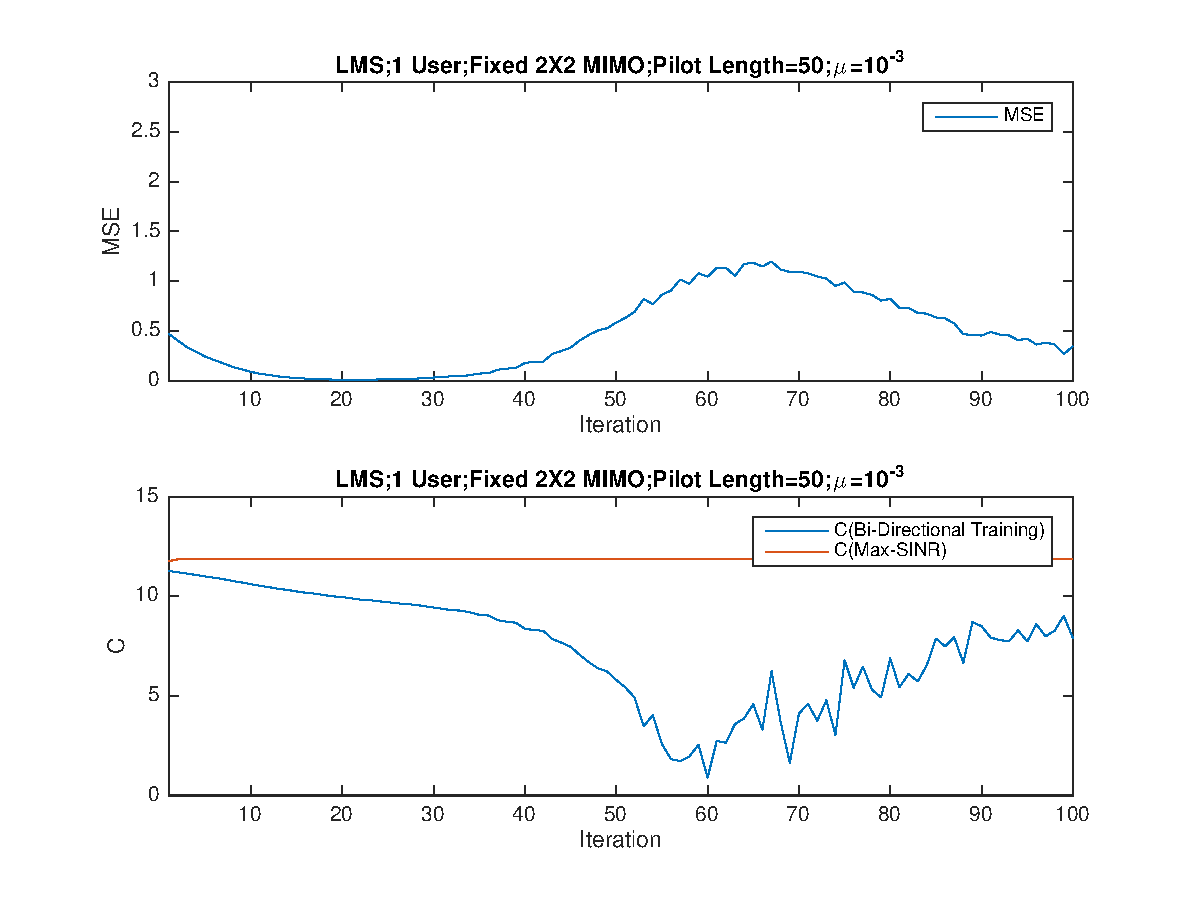
\includegraphics[width=220mm]{LMS1}}
    \caption{Insert caption}
\end{figure} 

\begin{figure}[bp!]
    \centering
    \centerline{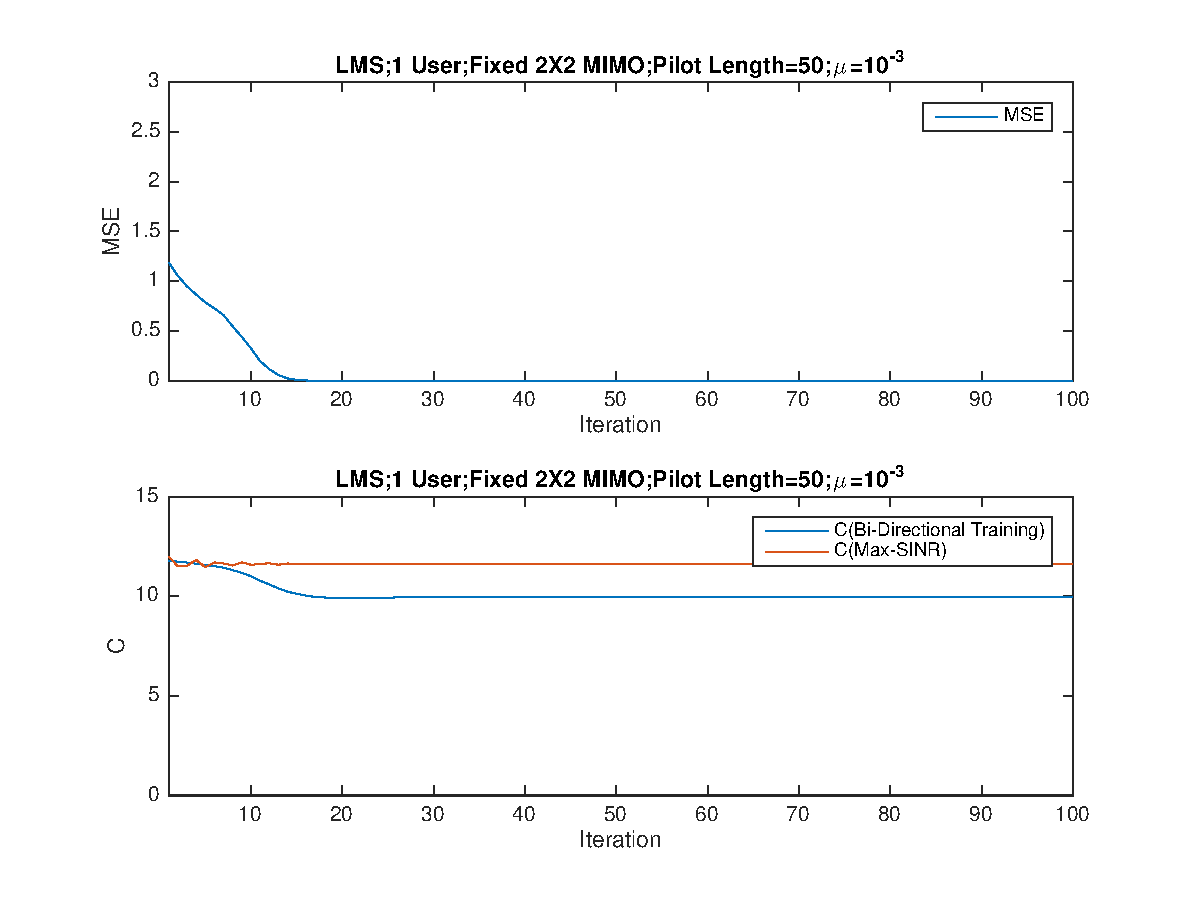
\includegraphics[width=220mm]{LMS2}}
    \caption{Insert caption}
\end{figure} 

\begin{figure}[bp!]
    \centering
    \centerline{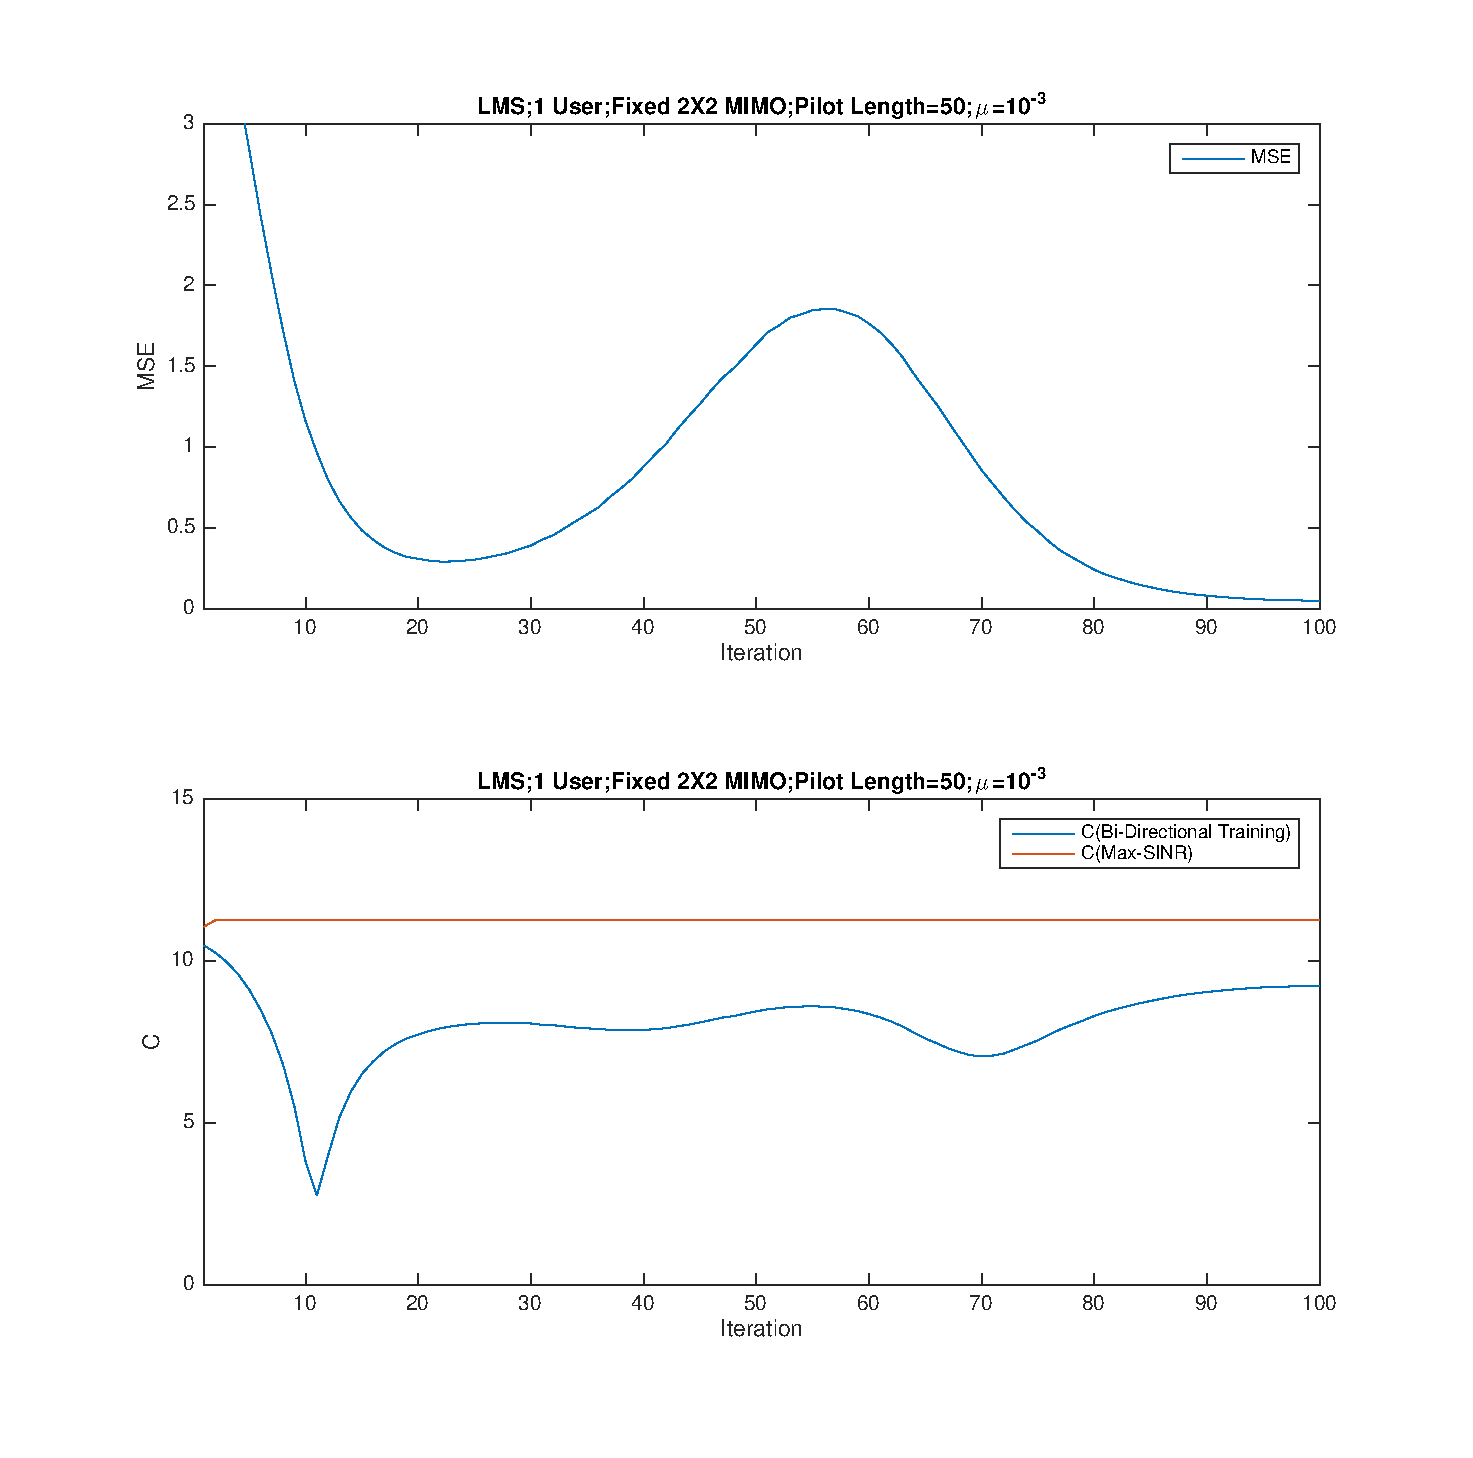
\includegraphics[width=220mm]{LMS3}}
    \caption{Insert caption}
\end{figure} 

\begin{figure}[bp!]
    \centering
    \centerline{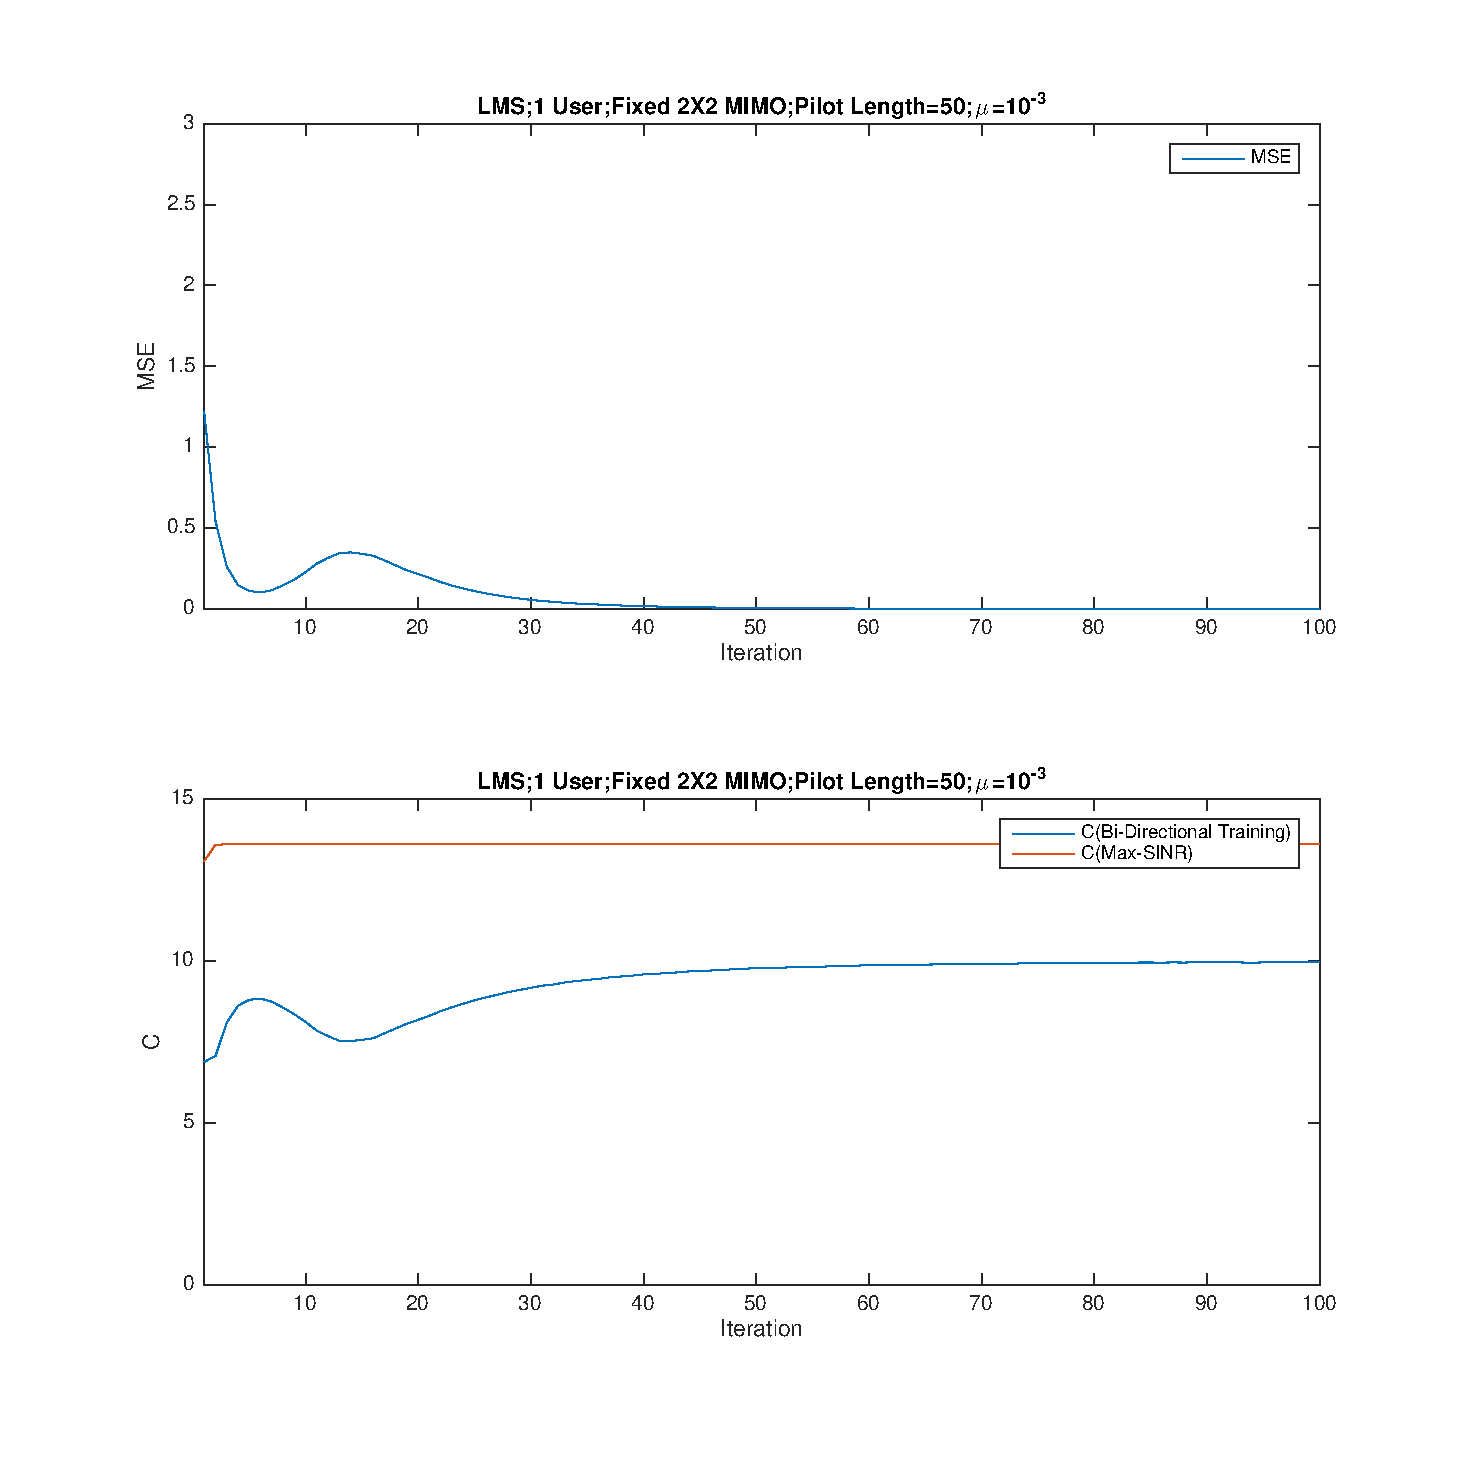
\includegraphics[width=220mm]{LMS4}}
    \caption{Insert caption}
\end{figure} 

\begin{figure}[bp!]
    \centering
    \centerline{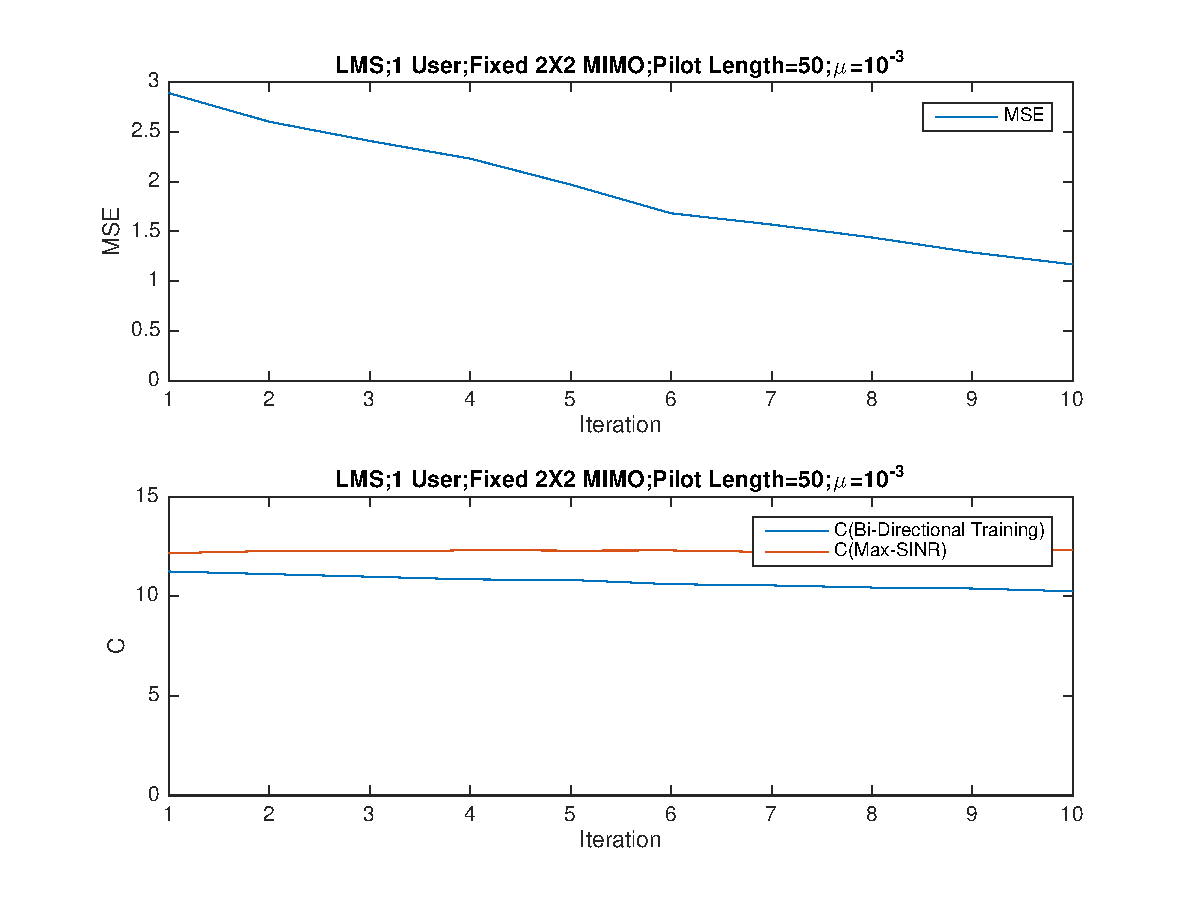
\includegraphics[width=220mm]{LMS5}}
    \caption{Insert caption}
\end{figure} 

\begin{figure}[bp!]
    \centering
    \centerline{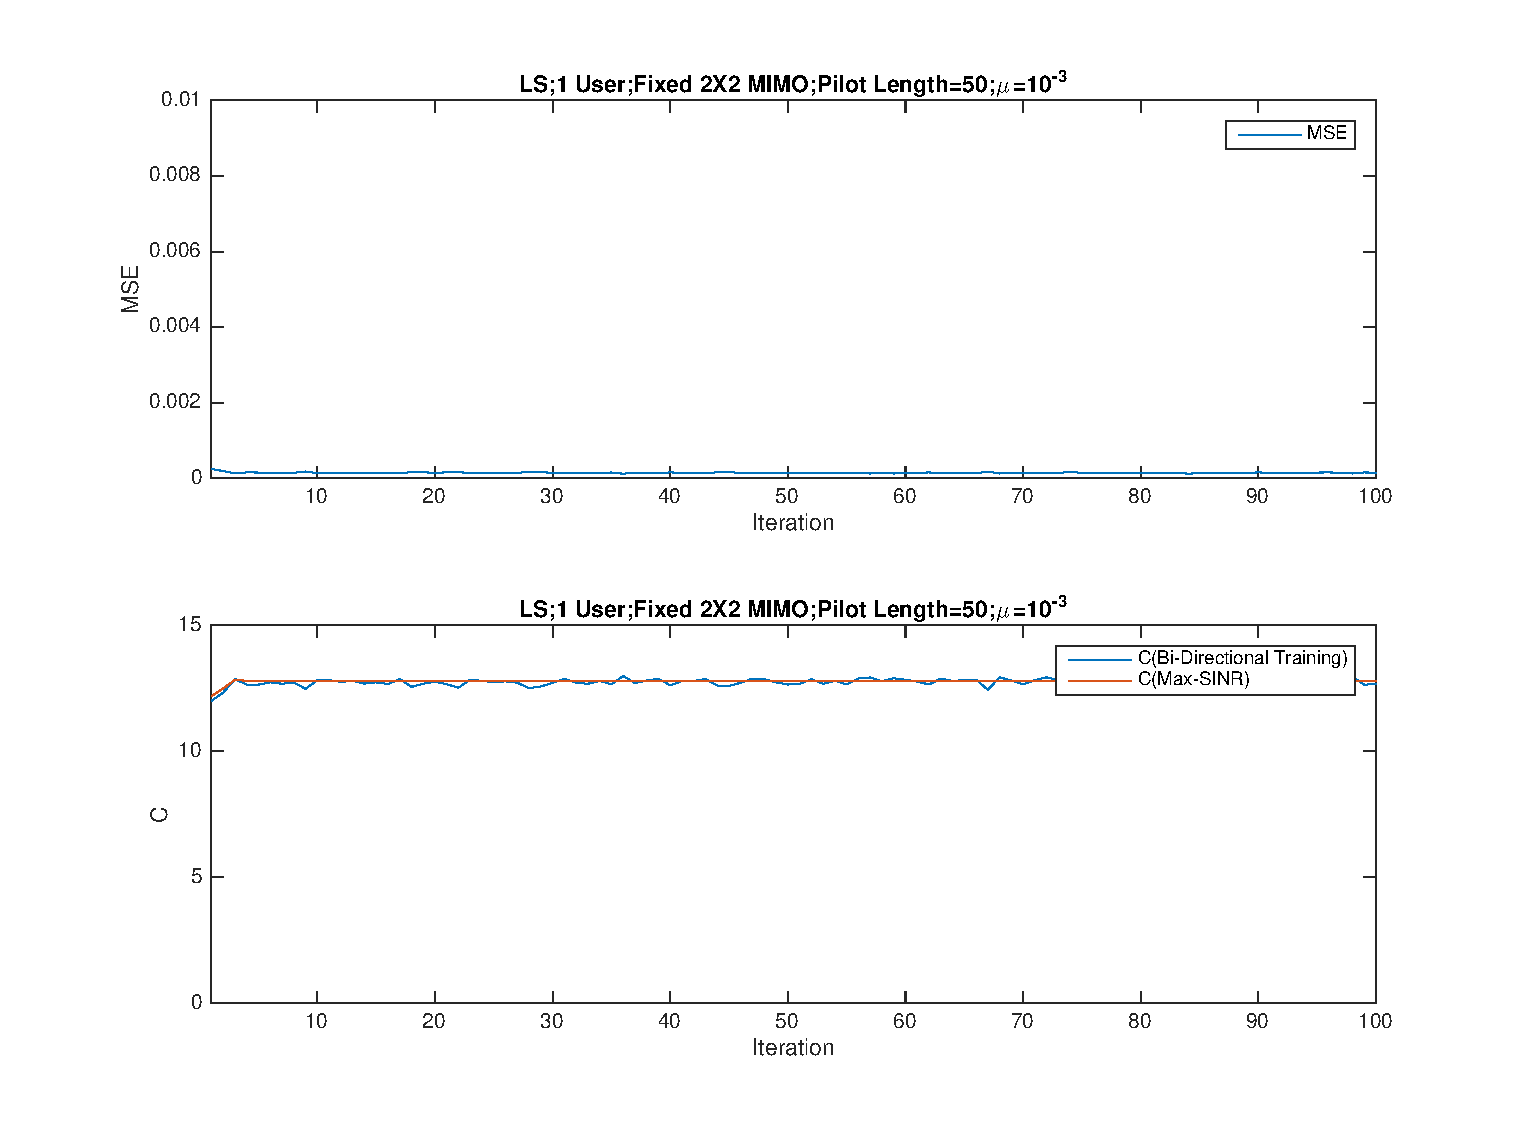
\includegraphics[width=220mm]{LS1}}
    \caption{Insert caption}
\end{figure} 

\begin{figure}[bp!]
    \centering
    \centerline{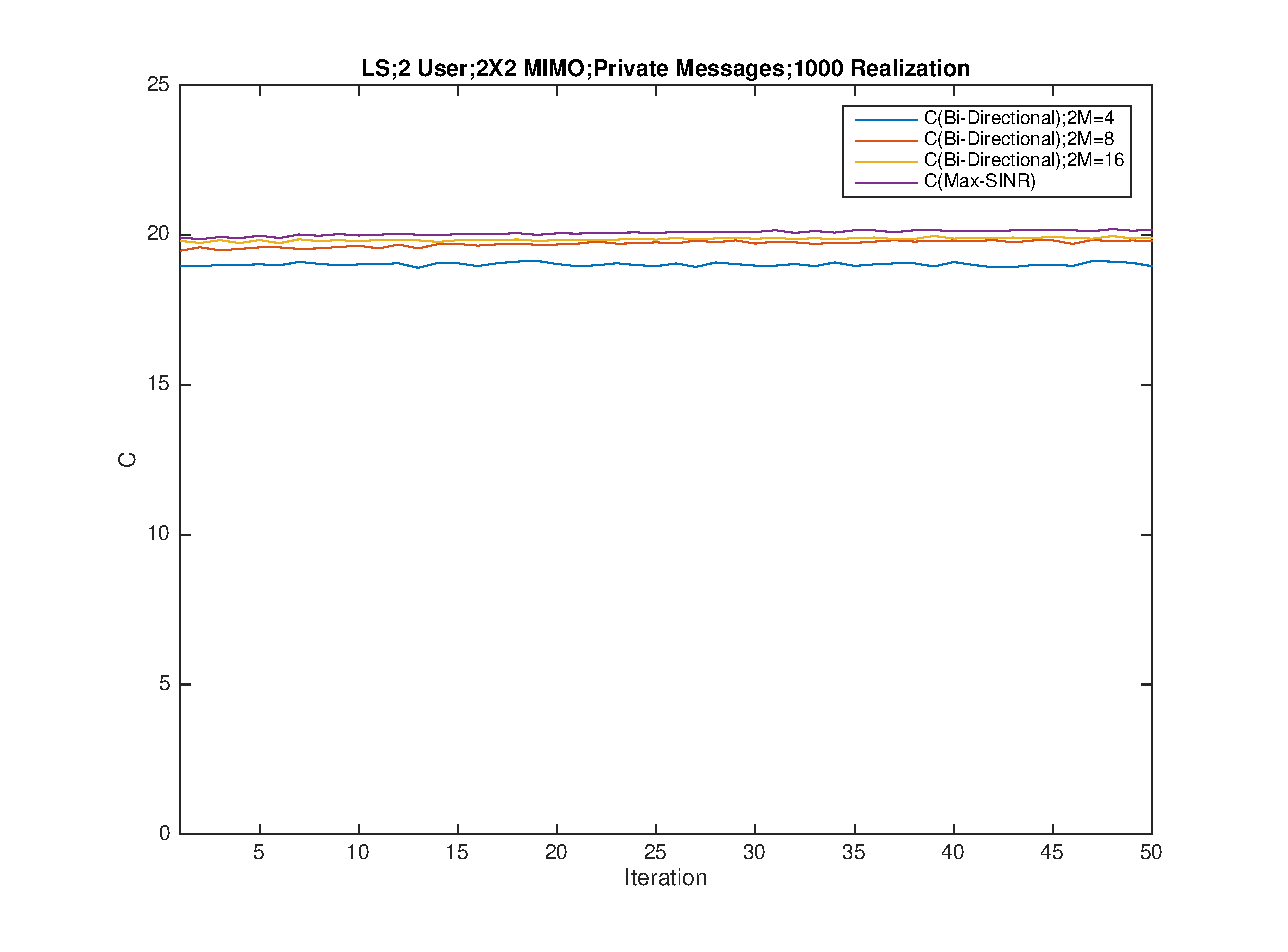
\includegraphics[width=220mm]{only_private}}
    \caption{Insert caption}
\end{figure} 

\begin{figure}[bp!]
    \centering
    \centerline{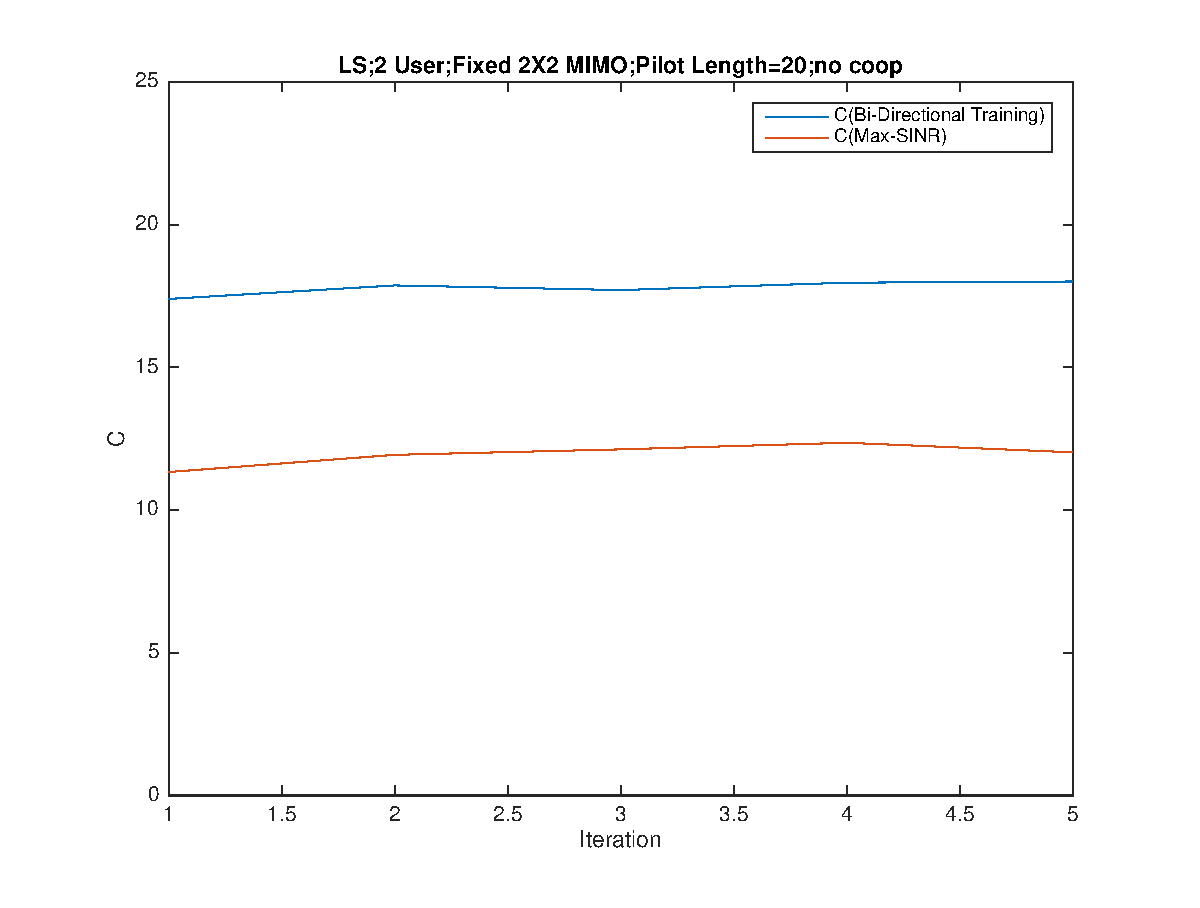
\includegraphics[width=220mm]{no_coop}}
    \caption{Insert caption}
\end{figure} 

\begin{figure}[bp!]
    \centering
    \centerline{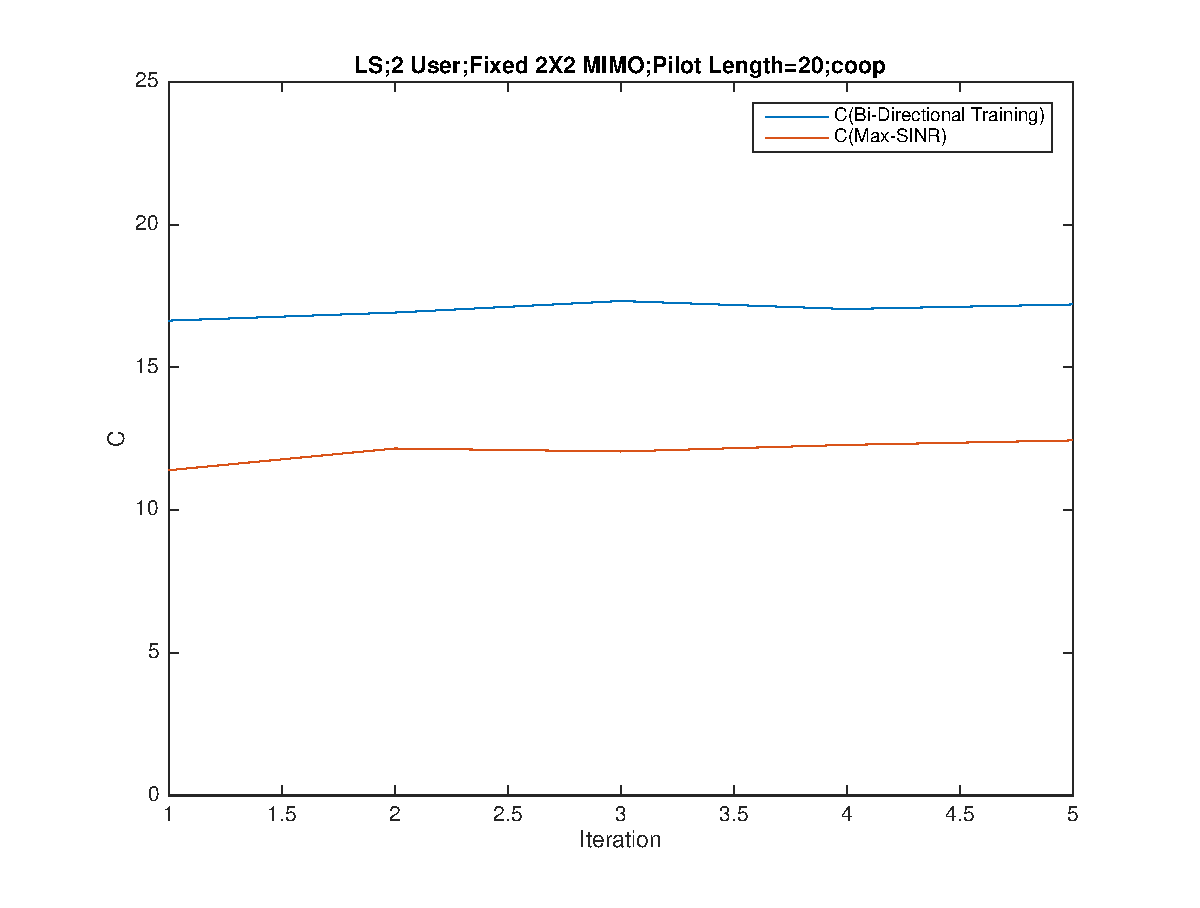
\includegraphics[width=220mm]{coop}}
    \caption{Insert caption}
\end{figure} 

 


\end{document}  